\section{Cơ sở lý thuyết}
\subsection{Giới thiệu về học máy(Machine learning)}
\indent Học máy (machine learning) là một lĩnh vực của trí tuệ nhân tạo liên quan đến việc nghiên cứu và xây dựng các kĩ thuật cho phép các hệ thống "học" tự động từ dữ liệu để giải quyết những vấn đề cụ thể. Lịch sử học máy bắt đầu từ những năm 1950 với các nỗ lực đầu tiên để mô phỏng khả năng học của con người thông qua máy tính. Tuy nhiên, cho đến đầu thập kỷ 21, học máy mới trở nên phổ biến và mạnh mẽ nhờ vào sự tiến bộ của phần cứng và khả năng tính toán.

\indent Trong thập kỷ gần đây, sự phát triển của các thuật toán học máy, kết hợp với dữ liệu lớn và sức mạnh tính toán ngày càng tăng, đã đưa học máy vào tầm tay của nhiều người và ứng dụng rộng rãi trong nhiều lĩnh vực, bao gồm nhận dạng hình ảnh, ngôn ngữ tự nhiên và IoT (Internet of Things).

\subsection{Giới thiệu về Mạng nơ-ron hồi quy(RNN)}
\subsubsection{Tổng quan}
\indent Mạng nơ-ron hồi quy (RNN) là một mô hình học sâu được đào tạo để xử lý và chuyển đổi đầu vào dữ liệu tuần tự thành đầu ra dữ liệu tuần tự cụ thể. Dữ liệu tuần tự là dữ liệu, chẳng hạn như từ, câu hoặc dữ liệu chuỗi thời gian, trong đó các thành phần tuần tự tương quan với nhau dựa trên ngữ nghĩa phức tạp và quy tắc cú pháp. RNN là một hệ thống phần mềm gồm nhiều thành phần được kết nối với nhau theo cách con người thực hiện chuyển đổi dữ liệu tuần tự, chẳng hạn như dịch văn bản từ ngôn ngữ này sang ngôn ngữ khác. Phần lớn RNN đang được thay thế bằng trí tuệ nhân tạo (AI) dựa trên công cụ biến đổi và các mô hình ngôn ngữ lớn (LLM), hiệu quả hơn nhiều trong việc xử lý dữ liệu tuần tự.
\begin{figure}[H]
    \centering
    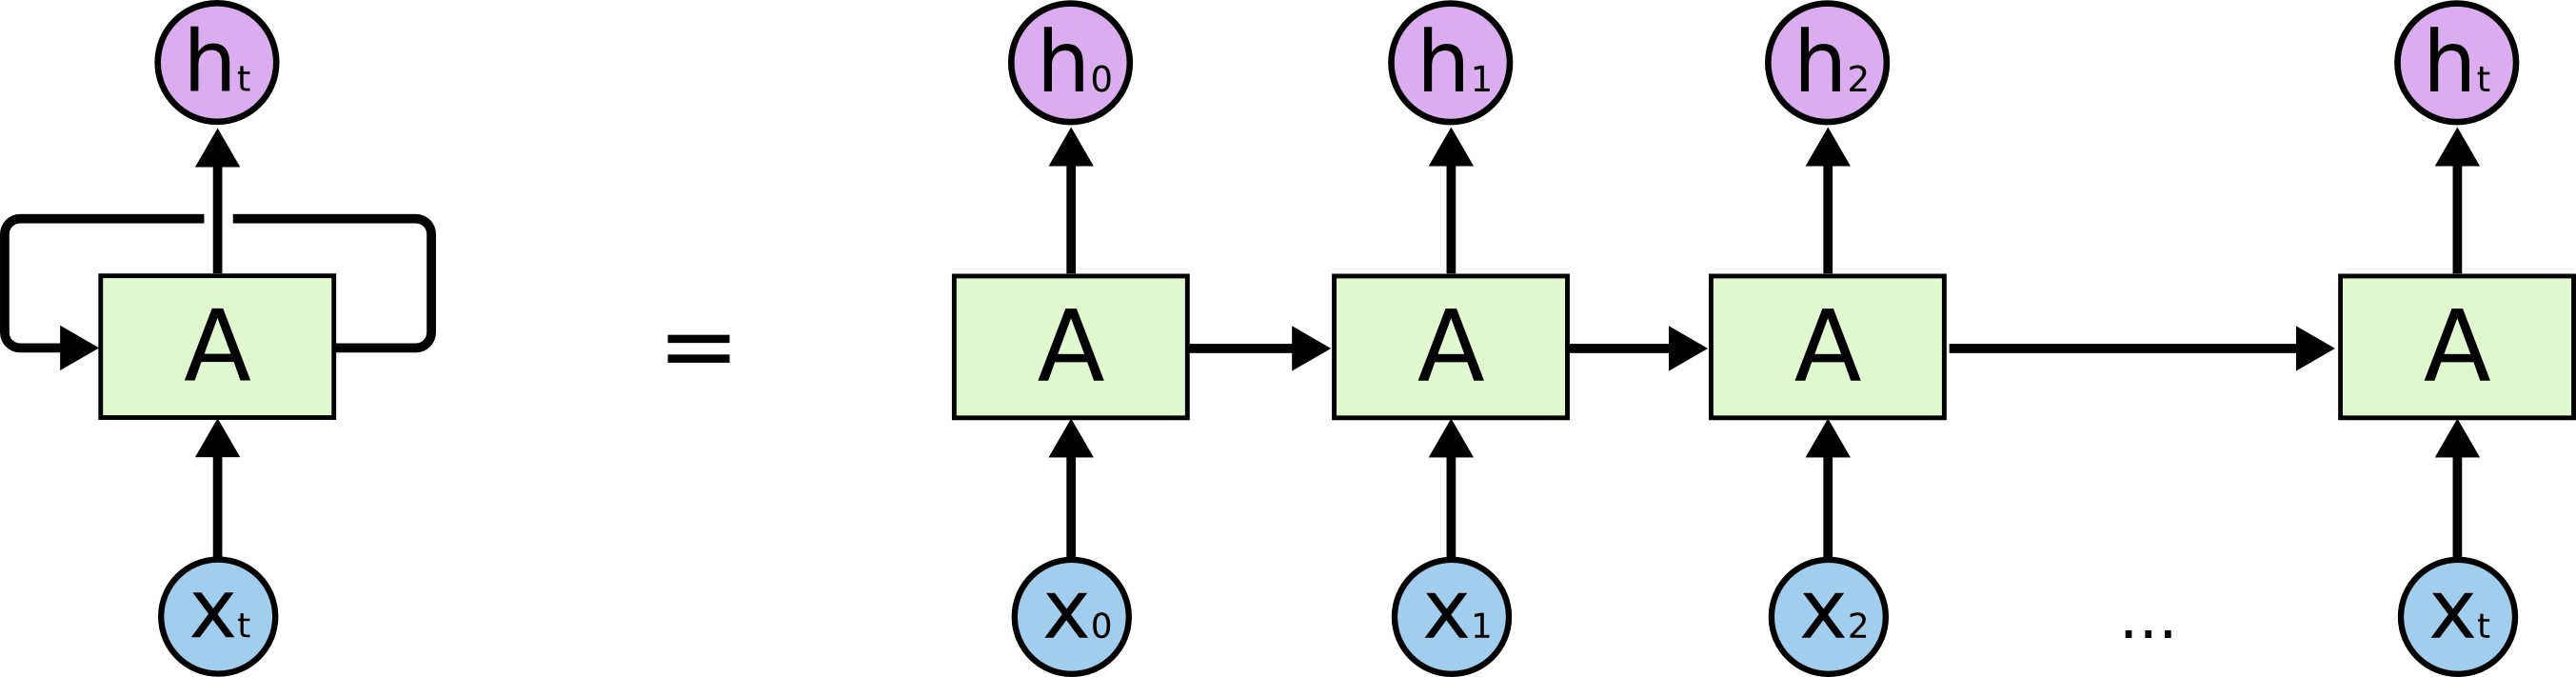
\includegraphics[width=\textwidth,height=\textheight,keepaspectratio]{Images/Theoretical basis/RNN-unrolled.png}
    \caption{Minh họa một mạng nơ-ron hồi quy}
    \label{fig:enter-label}
\end{figure}

\subsection{Một số loại nơ-ron hồi quy}
\indent RNN thường có đặc trưng là kiến trúc một-một: một chuỗi đầu vào được liên kết với một đầu ra. Tuy nhiên, bạn có thể điều chỉnh linh hoạt thành các cấu hình khác nhau cho các mục đích cụ thể. Sau đây là một số loại RNN phổ biến.
\begin{itemize}
    \item \textbf{Một-nhiều:} Loại RNN này dẫn một đầu vào đến một số đầu ra. Loại này tạo điều kiện cho các ứng dụng ngôn ngữ như chú thích hình ảnh bằng cách tạo một câu từ một từ khóa duy nhất.
    \item \textbf{Nhiều-nhiều:} Mô hình sử dụng nhiều đầu vào để dự đoán nhiều đầu ra. Ví dụ: bạn có thể tạo một công cụ dịch ngôn ngữ bằng RNN, với khả năng phân tích câu và cấu trúc chính xác các từ trong một ngôn ngữ khác.
    \item \textbf{Nhiều-một:} Một số đầu vào được ánh xạ đến một đầu ra. Loại này rất hữu ích trong các ứng dụng như phân tích cảm xúc, trong đó mô hình dự đoán cảm xúc của khách hàng như tích cực, tiêu cực và trung lập từ lời chứng thực đầu vào.
\end{itemize}

\begin{figure}[H]
    \centering
    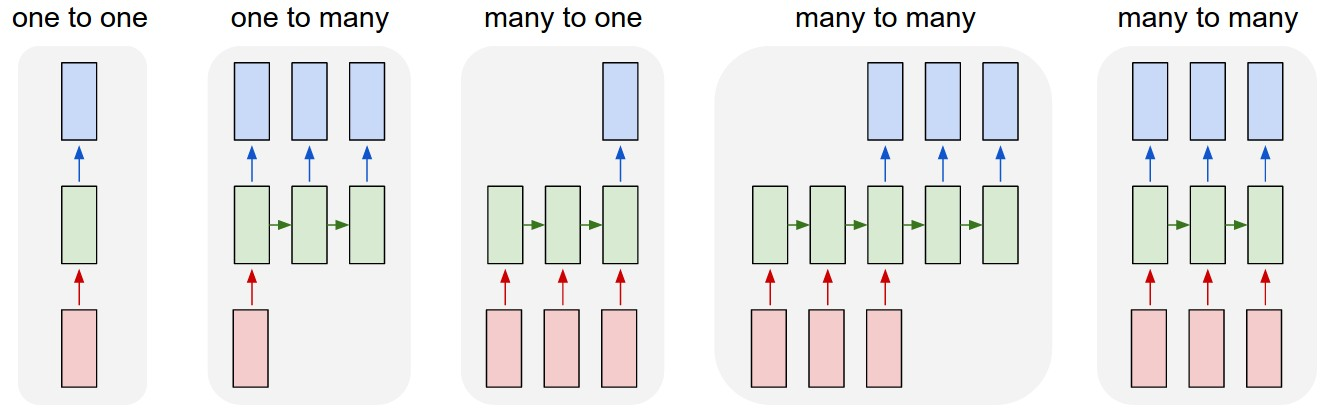
\includegraphics[width=\textwidth,height=\textheight,keepaspectratio]{Images/Theoretical basis/RNN_Type.jpeg}
    \caption{Một số kiểu nơ-ron hồi quy phổ biến}
    \label{fig:enter-label}
\end{figure}
\subsubsection{Vấn đề phụ thuộc xa của RNN}

\indent Một điểm nổi bật của RNN chính là ý tưởng kết nối các thông tin phía trước để dự đoán cho hiện tại. Việc này tương tự như ta sử dụng các cảnh trước của bộ phim để hiểu được cảnh hiện thời. Nếu mà RNN có thể làm được việc đó thì chúng sẽ cực kì hữu dụng, tuy nhiên liệu chúng có thể làm được không? Câu trả lời là còn tùy.

\indent Đôi lúc ta chỉ cần xem lại thông tin vừa có thôi là đủ để biết được tình huống hiện tại. Ví dụ, ta có câu: “các đám may trên bầu trời” thì ta chỉ cần đọc tới “các đám may trên bầu” là đủ biết được chữ tiếp theo là “trời” rồi. Trong tình huống này, khoảng cách tới thông tin có được cần để dự đoán là nhỏ, nên RNN hoàn toàn có thể học được.
\begin{figure}[H]
    \centering
    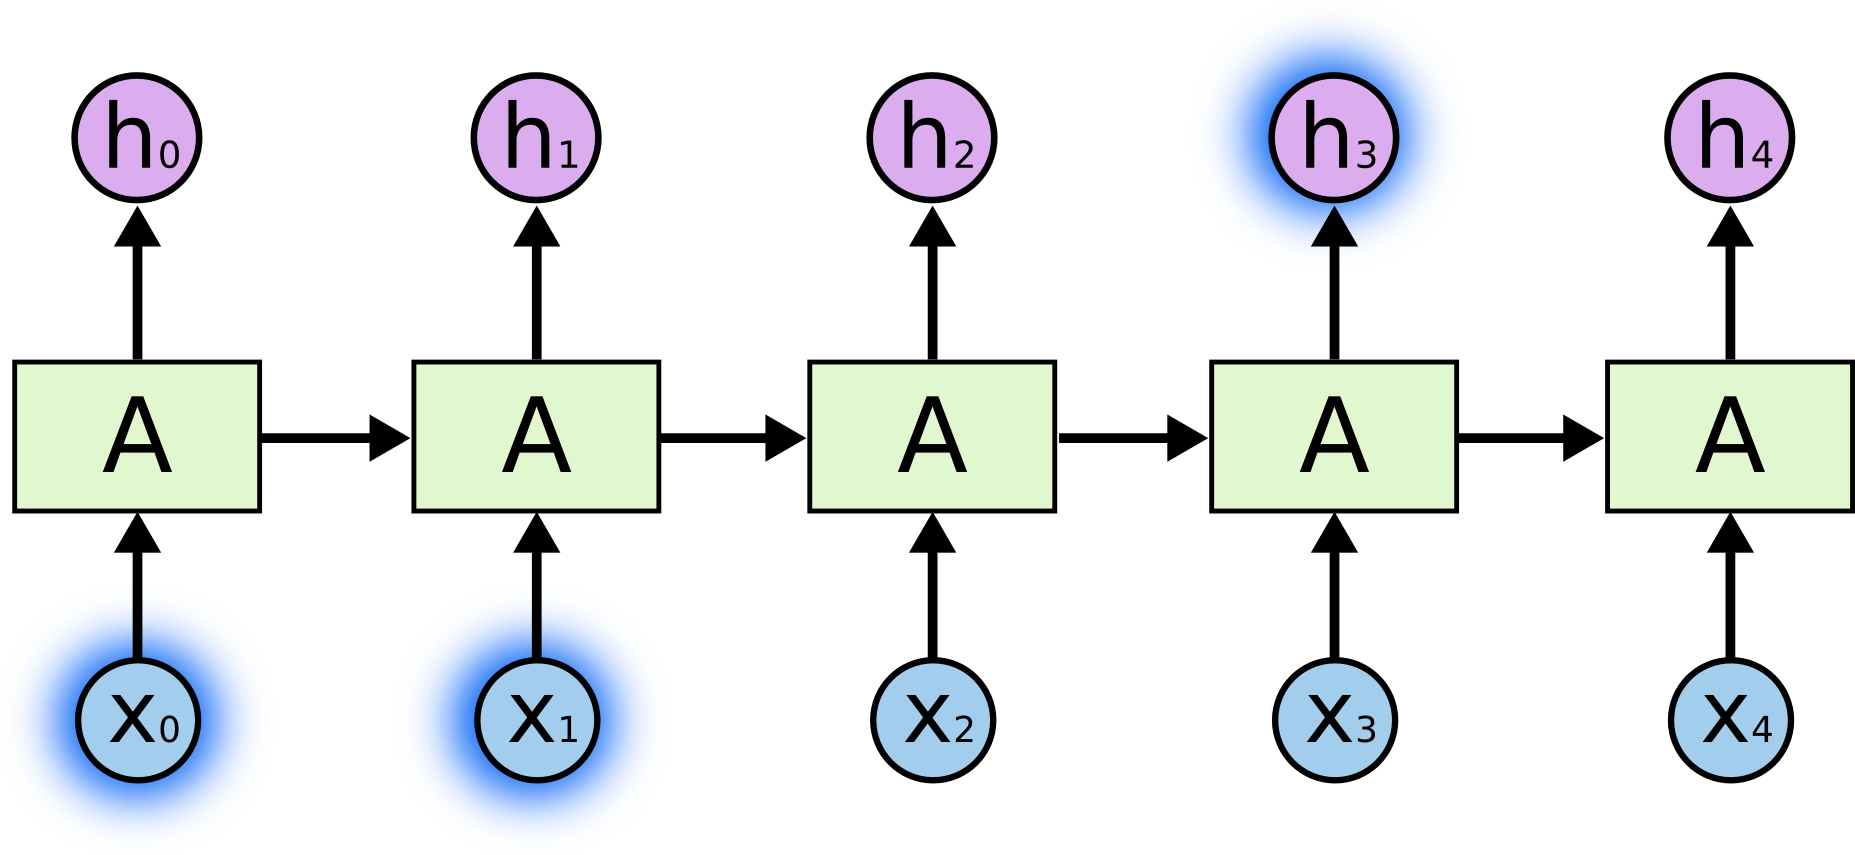
\includegraphics[width=\textwidth,height=\textheight,keepaspectratio]{Images/Theoretical basis/RNN-shorttermdepdencies.png}
    \caption{Phụ thuộc ngắn hạn trên RNN}
    \label{fig:enter-label}
\end{figure}
\indent Nhưng trong nhiều tình huống ta buộc phải sử dụng nhiều ngữ cảnh hơn để suy luận. Ví dụ, dự đoán chữ cuối cùng trong đoạn: “I grew up in France… I speak fluent French.”. Rõ ràng là các thông tin gần (”I speak fluent”) chỉ có phép ta biết được đằng sau nó sẽ là tên của một ngôn ngữ nào đó, còn không thể nào biết được đó là tiếng gì. Muốn biết là tiếng gì, thì ta cần phải có thêm ngữ cảnh “I grew up in France” nữa mới có thể suy luận được. Rõ ràng là khoảng cách thông tin lúc này có thể đã khá xa rồi.
\begin{figure}[H]
    \centering
    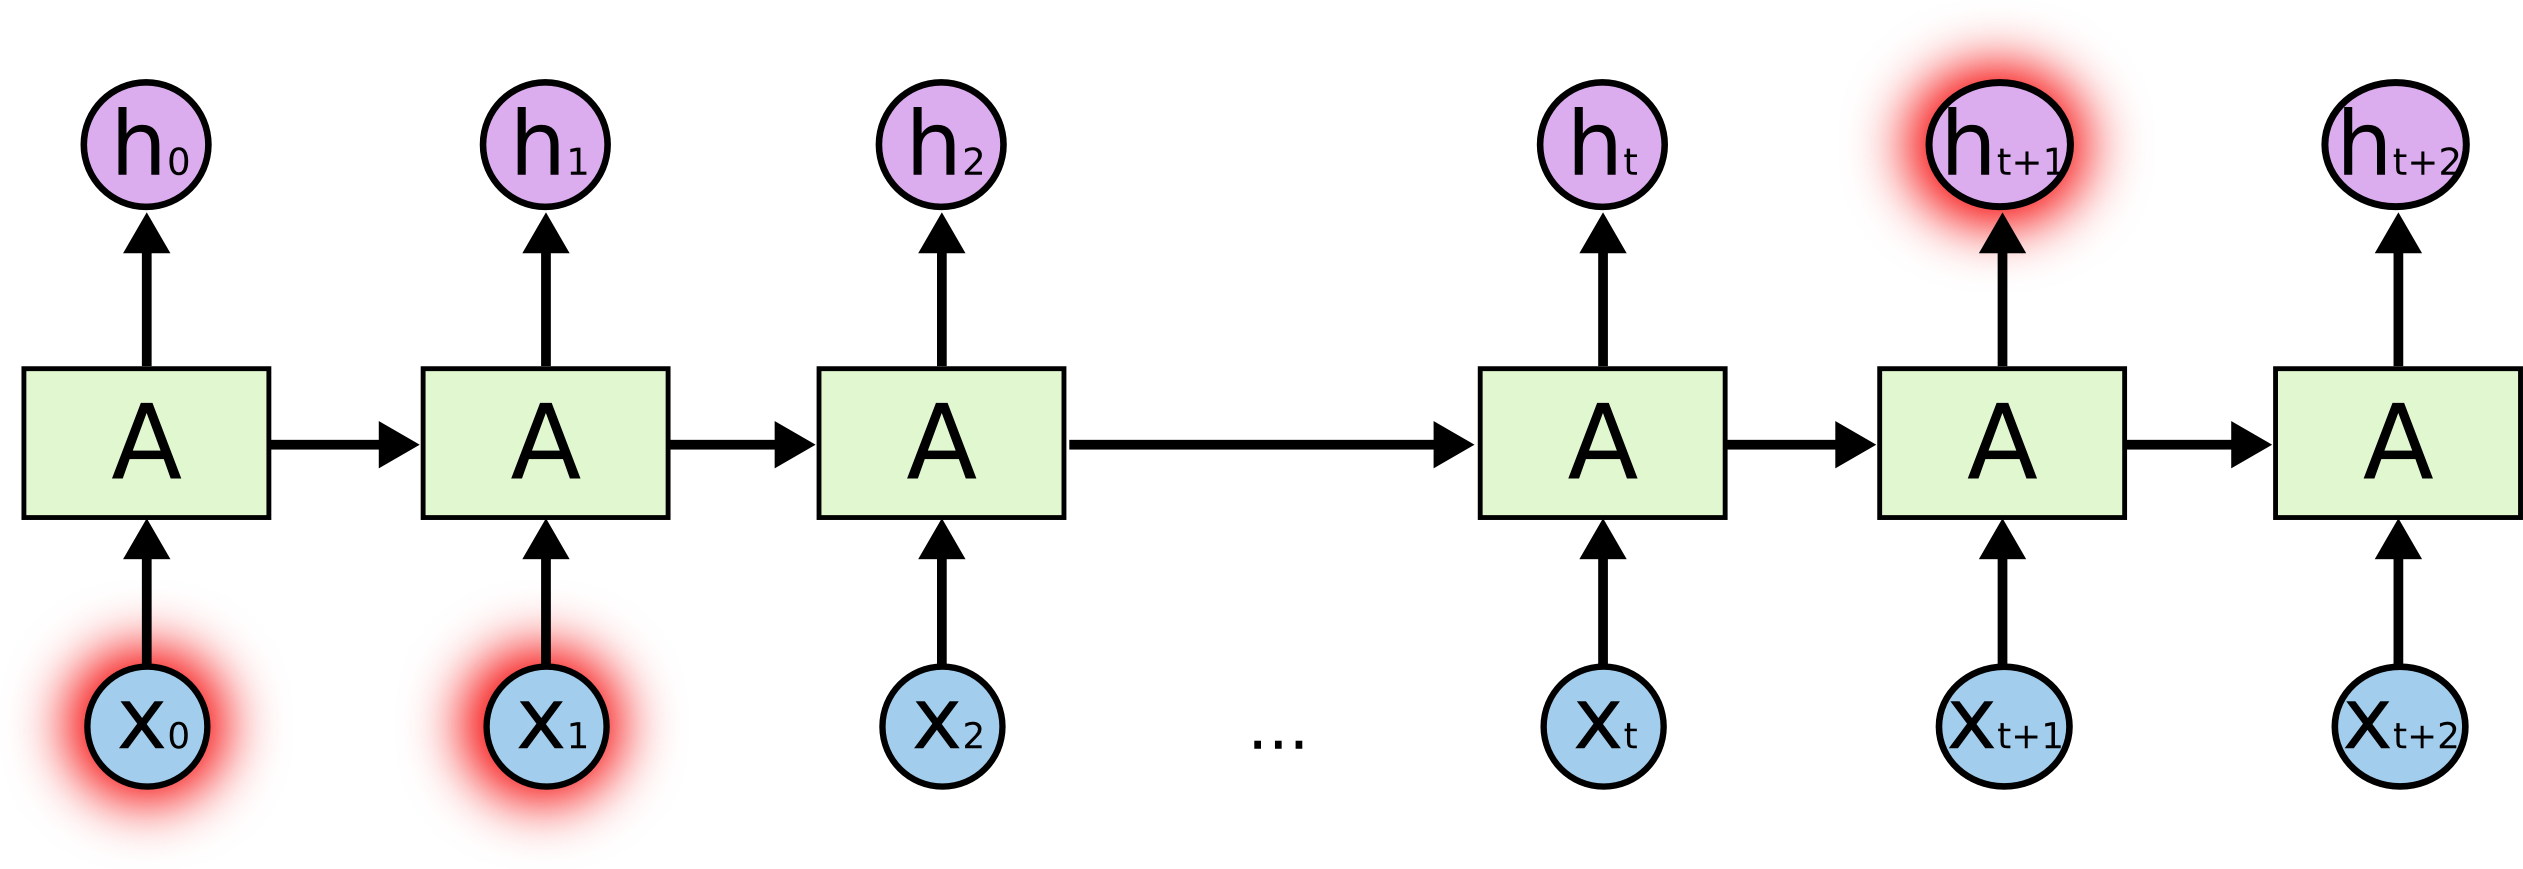
\includegraphics[width=\textwidth,height=\textheight,keepaspectratio]{Images/Theoretical basis/RNN-longtermdependencies.png}
    \caption{Phụ thuộc dài hạn trên RNN}
    \label{fig:enter-label}
\end{figure}
\indent Thật không may là với khoảng cách càng lớn dần thì RNN bắt đầu không thể nhớ và học được nữa.

\subsection{Giói thiệu mô hình Long-short term memmory(LTSM)}
\subsubsection{Giới thiệu tổng quan}

\indent Mạng bộ nhớ dài - ngắn (Long Short Term Memory networks), thường được gọi là LSTM - là một dạng đặc biệt của RNN, nó có khả năng học được các phụ thuộc xa. LSTM được giới thiệu bởi Hochreiter \& Schmidhuber vào năm 1997, và sau đó đã được cải tiến và phổ biến bởi rất nhiều người trong ngành. Chúng hoạt động cực kì hiệu quả trên nhiều bài toán khác nhau nên dần đã trở nên phổ biến như hiện nay.

\indent LSTM được thiết kế để tránh được vấn đề phụ thuộc xa (long-term dependency). Việc nhớ thông tin trong suốt thời gian dài là đặc tính mặc định của chúng, chứ ta không cần phải huấn luyện nó để có thể nhớ được. Tức là ngay nội tại của nó đã có thể ghi nhớ được mà không cần bất kì can thiệp nào.

\indent Mọi mạng hồi quy đều có dạng là một chuỗi các mô-đun lặp đi lặp lại của mạng nơ-ron. Với mạng RNN chuẩn, các mô-dun này có cấu trúc rất đơn giản, thường là một tầng tanh. LSTM cũng có kiến trúc dạng chuỗi như vậy, nhưng các mô-đun trong nó có cấu trúc khác với mạng RNN chuẩn. Thay vì chỉ có một tầng mạng nơ-ron, chúng có tới 4 tầng tương tác với nhau một cách rất đặc biệt.

\begin{figure}[H]
    \centering
    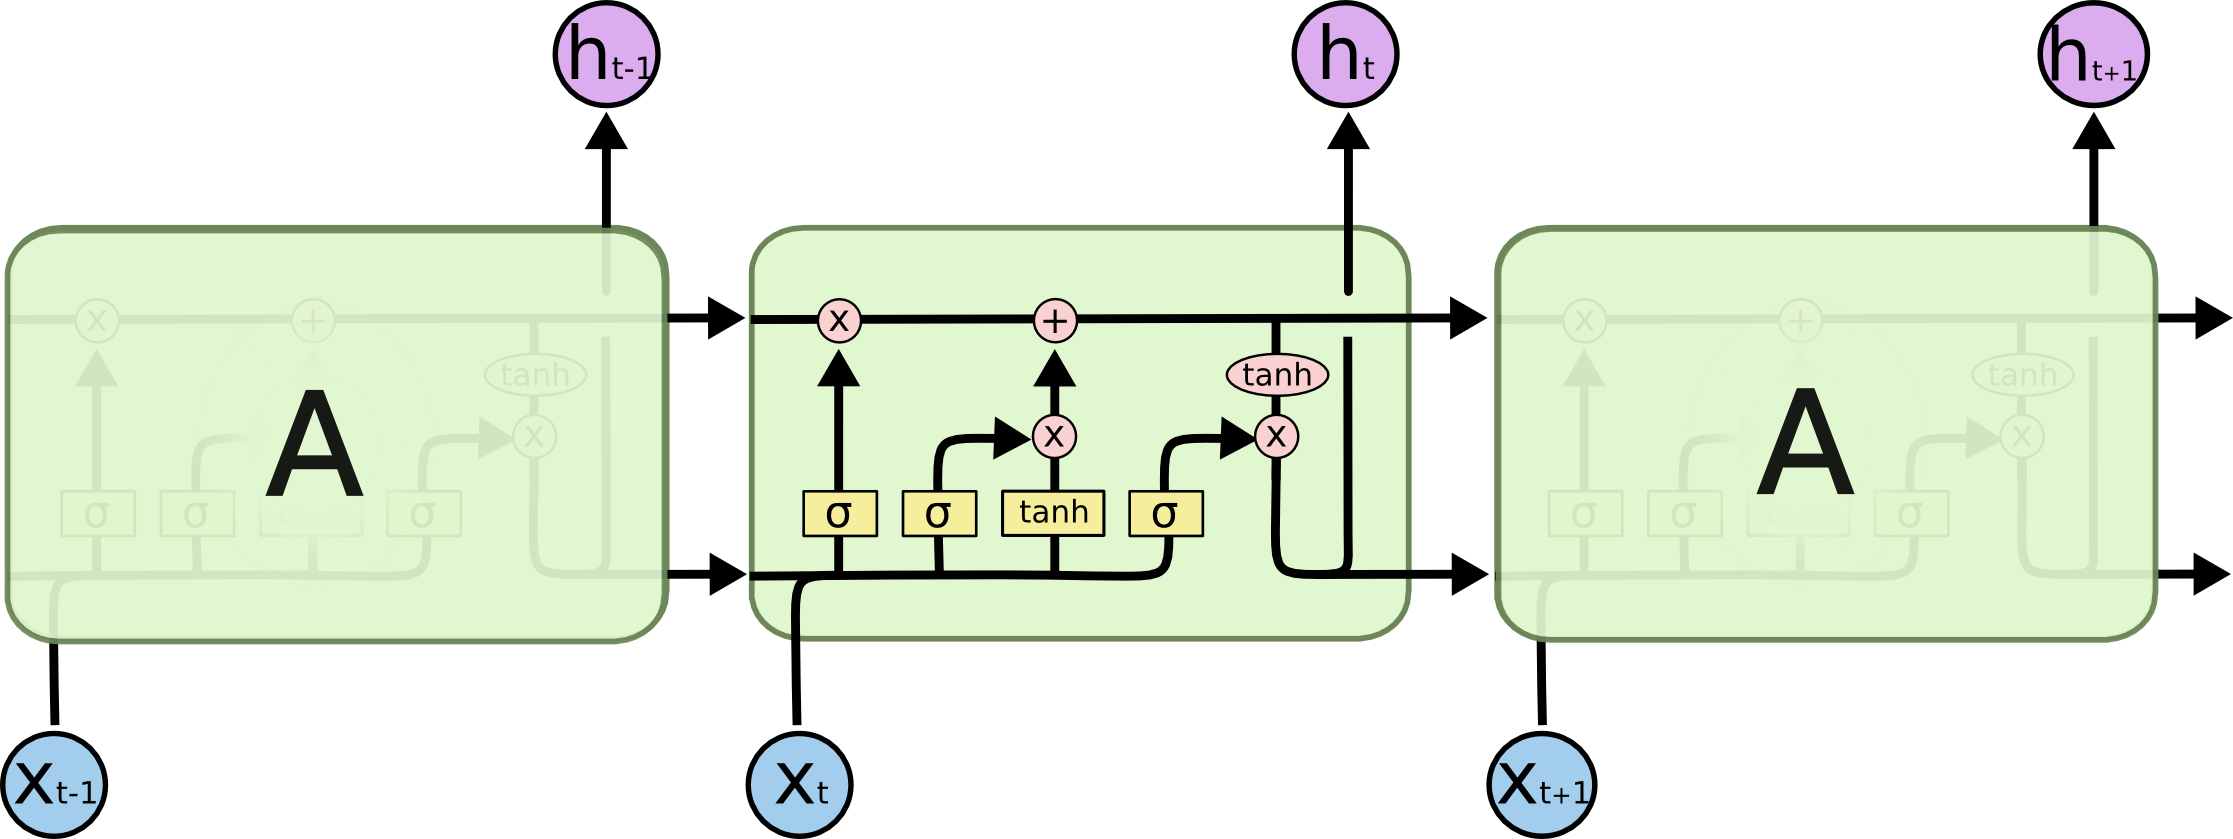
\includegraphics[width=14cm]{Images/Theoretical basis/LSTM.png}
\caption{Mô hình LSTM với 4 lớp tương tác}
\end{figure}
\subsubsection{Ý tưởng đằng sau LSTM}

\begin{figure}[H]
    \centering
    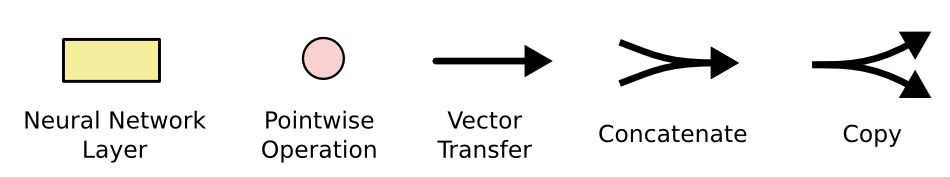
\includegraphics[width=14cm]{Images/Architecture/lstm1.png}
\caption{Diễn giải các kí hiệu trong đồ thị}
\end{figure}

\indent 

\begin{itemize}
    \item Ý tưởng chính của LSTM là thành phần ô trạng thái (cell state) được thể hiện qua đường chạy ngang qua đỉnh đồ thị như hình vẽ bên dưới:
    \begin{figure}[H]
        \centering
        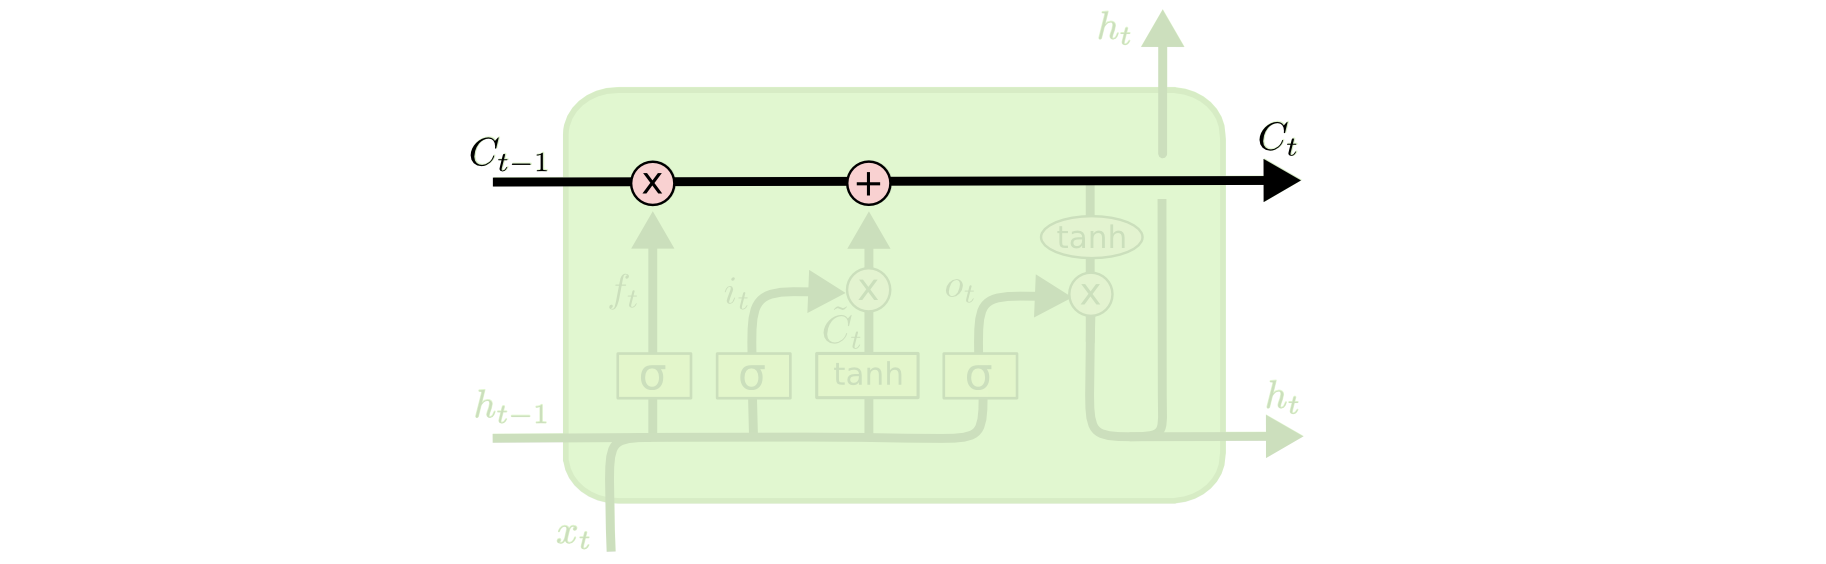
\includegraphics[width=14cm]{Images/Architecture/LSTM3-C-line.png}
    \caption{Đường đi của ô trạng thái (cell state) trong mạng LSTM}
    \end{figure}
    \item Ô trạng thái là một dạng băng chuyền chạy thẳng xuyên suốt toàn bộ chuỗi với chỉ một vài tương tác tuyến tính nhỏ giúp cho thông tin có thể truyền dọc theo đồ thị mạng nơ-ron ổn định.
    \item LSTM có khả năng xóa và thêm thông tin vào ô trạng thái và điều chỉnh các luồng thông tin này thông qua các cấu trúc gọi là cổng.
    \item Cổng là cơ chế đặc biệt để điều chỉnh luồng thông tin đi qua. Chúng được tổng hợp bởi một tầng ẩn của hàm activation sigmoid và với một toán tử nhân như đồ thị.
    \begin{figure}[H]
        \centering
        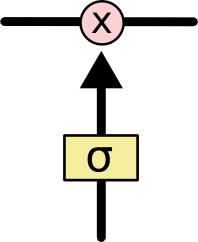
\includegraphics[width=3cm]{Images/Architecture/LSTM3-gate.png}
    \caption{Một cổng của hàm sigmoid trong LSTM}
    \end{figure}
    \item Hàm sigmoid sẽ cho đầu ra là một giá trị xác xuất nằm trong khoảng từ 0 đến 1, thể hiện rằng có bao nhiêu phần thông tin sẽ đi qua cổng. Giá trị bằng 0 ngụ ý rằng không cho phép thông tin nào đi qua, giá trị bằng 1 sẽ cho toàn bộ thông tin đi qua.
    \item Một mạng LSTM sẽ có 3 cổng có kiến trúc dạng này để bảo vệ và kiểm soát các ô trạng thái.
\end{itemize}

\subsubsection{Thứ tự các bước của LSTM}

\indent Bước đầu tiên trong LSTM sẽ quyết định xem thông tin nào chúng ta sẽ cho phép đi qua ô trạng thái (cell state). Nó được kiểm soát bởi hàm sigmoid trong một tầng gọi là tầng quên (forget gate layer). Đầu tiên nó nhận đầu vào là 2 giá trị \( h_{t-1} \)
 và \( x_{t} \)
 và trả về một giá trị nằm trong khoảng 0 và 1 cho mỗi giá trị của ô trạng thái \( \text{C}_{t-1} \)
. Nếu giá trị bằng 1 thể hiện ‘giữ toàn bộ thông tin’ và bằng 0 thể hiện ‘bỏ qua toàn bộ chúng’.

\indent Trở lại ví dụ về ngôn ngữ, chúng ta đang cố gắng dự báo từ tiếp theo dựa trên toàn bộ những từ trước đó. Trong những bài toán như vậy, ô trạng thái có thể bao gồm loại của chủ ngữ hiện tại, để cho đại từ ở câu tiếp theo được sử dụng chính xác. Chẳng hạn như chúng ta đang mô tả về một người bạn là con trai thì các đại từ nhân xưng ở tiếp theo phải là anh, thằng, hắn thay vì cô, con ấy. Tuy nhiên chủ ngữ không phải khi nào cũng cố định. Khi chúng ta nhìn thấy một chủ ngữ mới, chúng ta muốn quên đi loại của một chủ ngữ cũ. Do đó tầng quên cho phép cập nhật thông tin mới và lưu giữ giá trị của nó khi có thay đổi theo thời gian.

\begin{figure}[H]
    \centering
    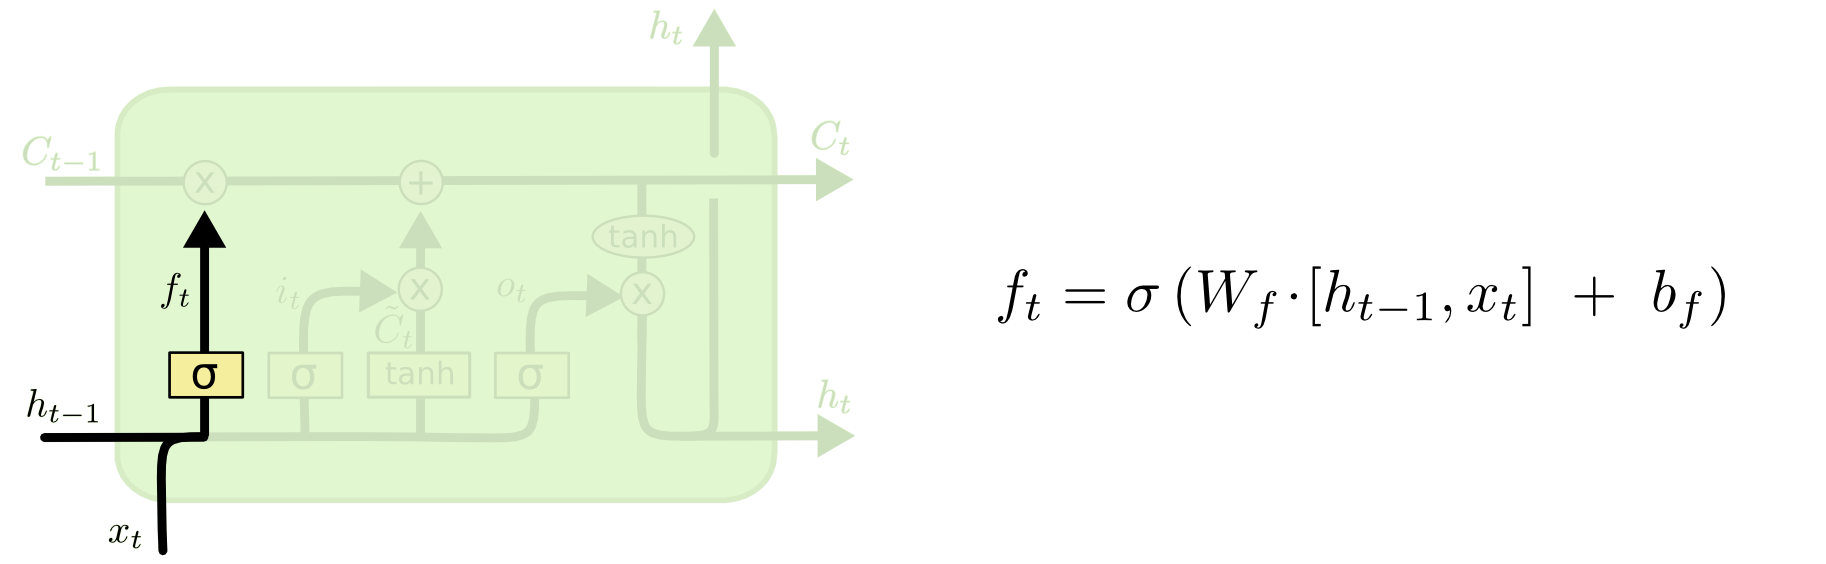
\includegraphics[width=14cm]{Images/Architecture/LSTM3-focus-f.png}
\caption{Tầng cổng quên (forget gate layer)}
\end{figure}

\indent Bước tiếp theo chúng ta sẽ quyết định loại thông tin nào sẽ được lưu trữ trong ô trạng thái. Bước này bao gồm 2 phần. Phần đầu tiên là một tầng ẩn của hàm sigmoid được gọi là tầng cổng vào (input gate layer) quyết định giá trị bao nhiêu sẽ được cập nhật. Tiếp theo, tầng ẩn hàm tanh sẽ tạo ra một véc tơ của một giá trị trạng thái mới 
 mà có thể được thêm vào trạng thái. Tiếp theo kết hợp kết quả của 2 tầng này để tạo thành một cập nhật cho trạng thái.

 \indent Trong ví dụ của mô hình ngôn ngữ, chúng ta muốn thêm loại của một chủ ngữ mới vào ô trạng thái để thay thế phần trạng thái cũ muốn quên đi.

\begin{figure}[H]
    \centering
    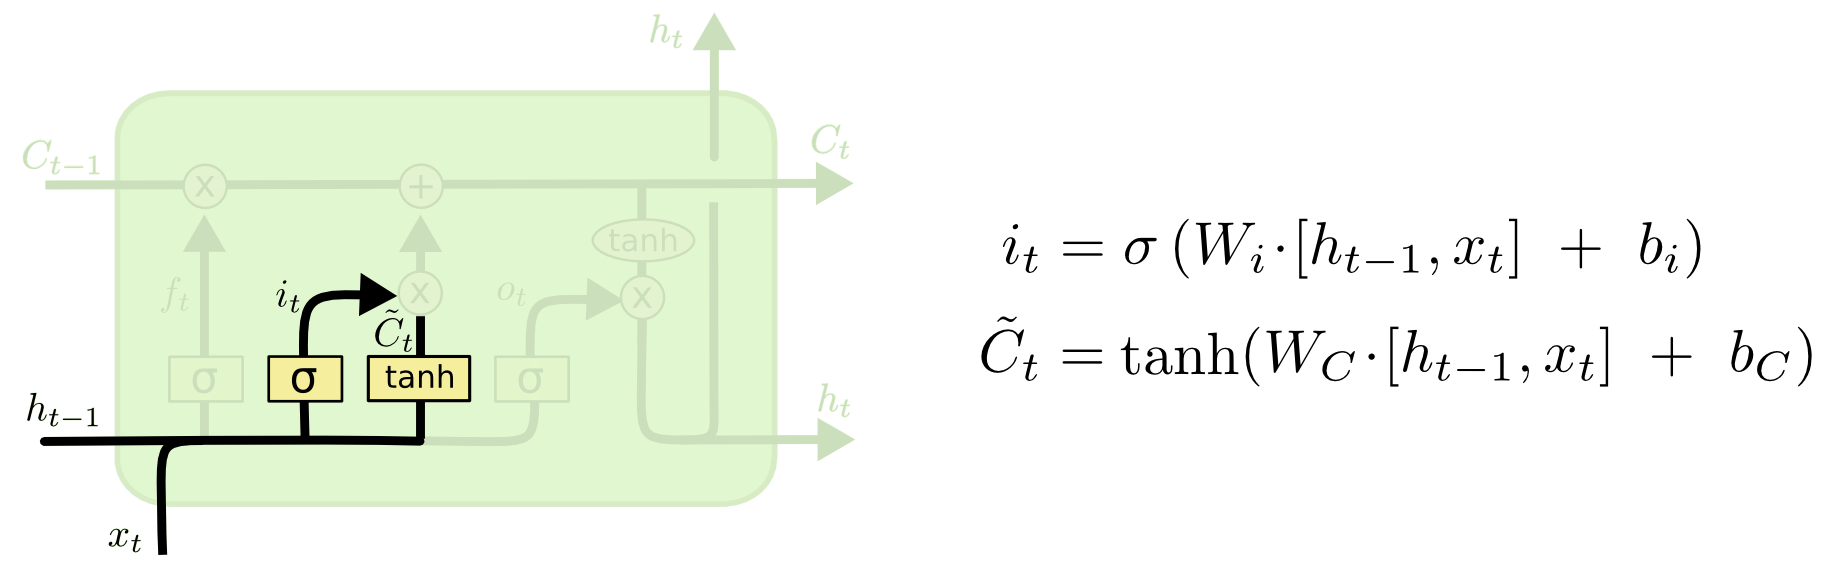
\includegraphics[width=14cm]{Images/Architecture/LSTM3-focus-i.png}
\caption{ Cập nhật giá trị cho ô trạng thái bằng cách kết hợp 2 kết quả từ tầng cổng vào và tẩng ẩn hàm tanh}
\end{figure}

\indent Đây là thời điểm để cập nhật một ô trạng thái cũ \( \text{C}_{t-1} \)
 sang một trạng thái mới \( \text{C}_{t} \)
. Những bước trước đó đã quyết định làm cái gì, và tại bước này chỉ cần thực hiện nó.

\indent Chúng ta nhân trạng thái cũ với \( f_{t} \)
 tương ứng với việc quên những thứ quyết định được phép quên sớm. Phần tử đề cử \( \tilde{\text{C}}_{t-1} \)
 là một giá trị mới được tính toán tương ứng với bao nhiêu được cập nhật vào mỗi giá trị trạng thái.

 \begin{figure}[H]
    \centering
    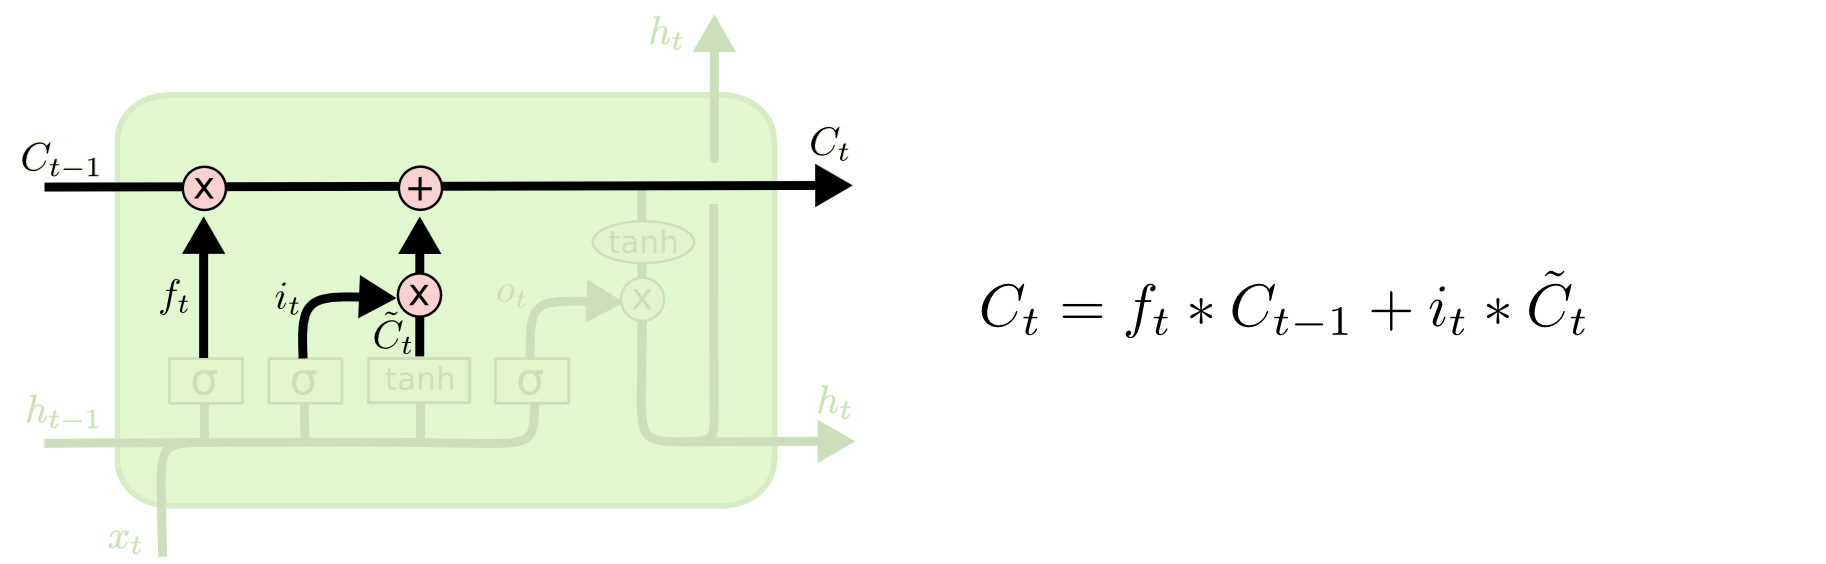
\includegraphics[width=14cm]{Images/Architecture/LSTM3-focus-C.png}
\caption{Ô trạng thái mới}
\end{figure}

\indent Cuối cùng cần quyết định xem đầu ra sẽ trả về bao nhiêu. Kết quả ở đầu ra sẽ dựa trên ô trạng thái, nhưng sẽ là một phiên bản được lọc. Đầu tiên, chúng ta chạy qua một tầng sigmoid nơi quyết định phần nào của ô trạng thái sẽ ở đầu ra. Sau đó, ô trạng thái được đưa qua hàm tanh (để chuyển giá trị về khoảng -1 và 1) và nhân nó với đầu ra của một cổng sigmoid, do đó chỉ trả ra phần mà chúng ta quyết định.

 \begin{figure}[H]
    \centering
    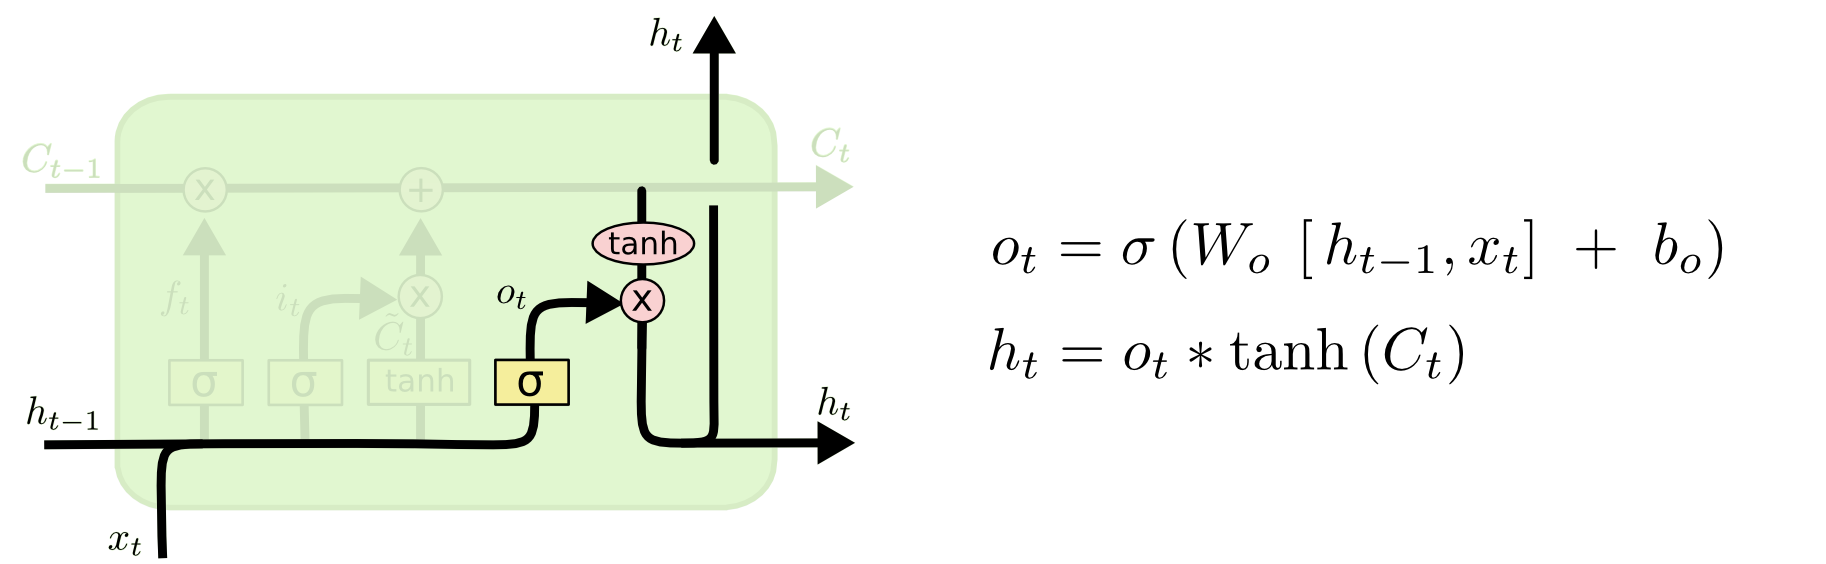
\includegraphics[width=14cm]{Images/Architecture/LSTM3-focus-o.png}
\caption{Điều chỉnh thông tin ở đầu ra thông qua hàm tanh}
\end{figure}
\subsubsection{Ưu và nhược điểm của mô hình LSTM}

\begin{enumerate}[-]
    \item Ưu điểm
    \begin{itemize}
        \item LSTM được thiết kế để xử lý dữ liệu chuỗi và giữ thông tin từ quá khứ, giúp nó phù hợp cho nhiều loại dự đoán chuỗi như ngôn ngữ tự nhiên, dự đoán chuỗi thời gian, v.v.
        \item LSTM có khả năng học và giữ lại thông tin lâu dài, giúp chúng phát hiện và theo dõi các mối quan hệ phức tạp trong dữ liệu dài hạn.
        \item LSTM sử dụng cổng quên (forget gate) để kiểm soát việc giữ và quên thông tin, giúp giảm hiện tượng triệt tiêu gradient, vấn đề thường gặp trong các mô hình RNN.
        \item Có thể kết hợp nhiều lớp LSTM để tạo thành các mô hình học sâu phức tạp hơn, linh hoạt trong việc xử lý nhiều loại dữ liệu và nhiều mức độ phức tạp.
    \end{itemize}
    \item  Nhược điểm
    \begin{itemize}
        \item Mô hình LSTM có khả năng tính toán khá phức tạp, đặc biệt khi được sử dụng trong các mô hình lớn với nhiều tham số.
        \item Do tính toán phức tạp, việc huấn luyện mô hình LSTM có thể mất nhiều thời gian, đặc biệt là khi làm việc với dữ liệu lớn.
        \item Mô hình LSTM có nguy cơ cao về overfitting, đặc biệt khi kích thước dữ liệu huấn luyện ít và mô hình quá phức tạp.
        \item Mặc dù LSTM giảm vấn đề triệt tiêu gradient, nhưng không giải quyết hoàn toàn vấn đề gradient exploding.
    \end{itemize}
\end{enumerate}
\subsection{Giới thiệu về Transfer Learning}

Transfer learning (học chuyển giao) là một kỹ thuật học máy trong đó một mô hình được phát triển cho một nhiệm vụ được sử dụng lại như là điểm khởi đầu cho một mô hình trên một nhiệm vụ thứ hai. Nói cách khác, kiến thức thu được trong khi giải quyết một vấn đề được áp dụng cho một vấn đề khác, nhưng có liên quan. 

\subsubsection{Định nghĩa Transfer Learning}

Transfer learning là việc sử dụng kiến thức đã học từ một miền nguồn (source domain) để cải thiện việc học trong một miền đích (target domain) khác. Miền nguồn thường có lượng dữ liệu lớn hơn và/hoặc dễ học hơn miền đích. 

 \begin{figure}[H]
    \centering
    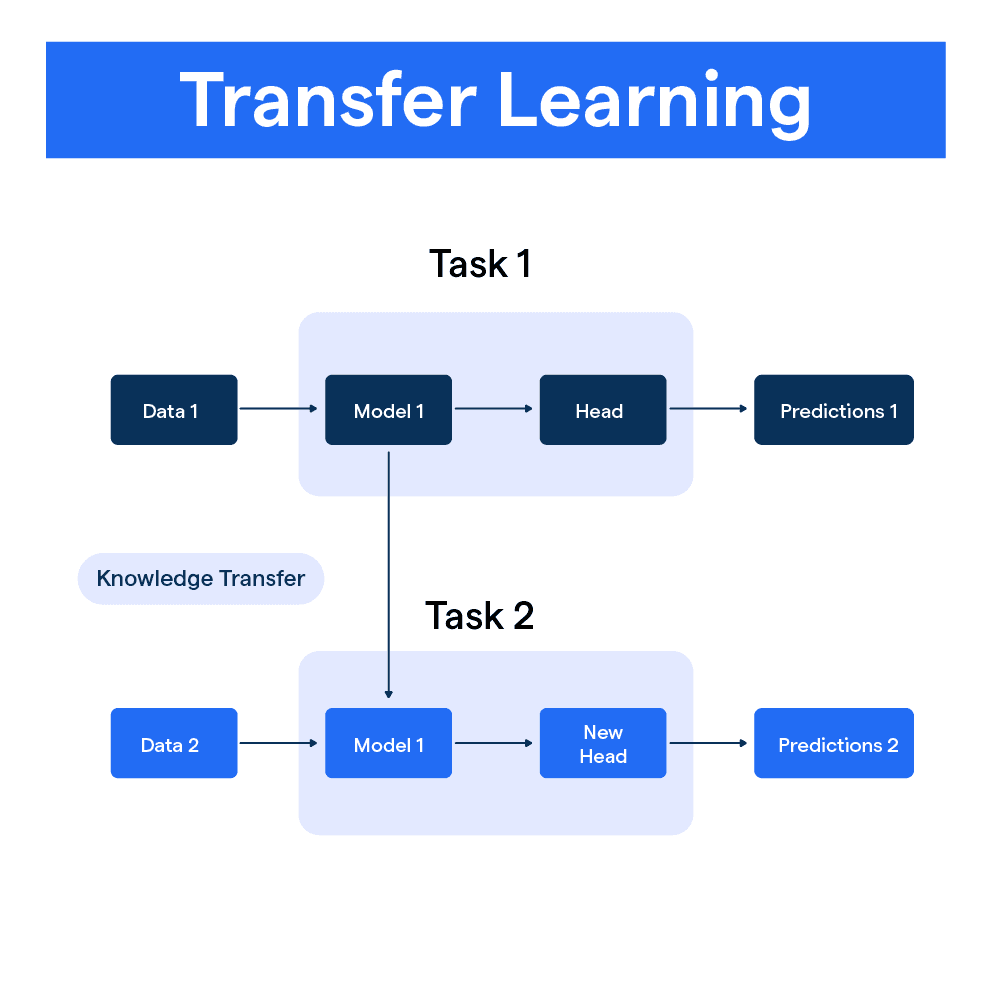
\includegraphics[width=10cm]{Images/Theoretical basis/Transfer_Learning.png}
\caption{Transfer learning}
\end{figure}


\subsubsection{Ứng dụng của Transfer Learning}

Transfer learning đã được ứng dụng thành công trong nhiều lĩnh vực, bao gồm:

\begin{itemize}
    \item \textbf{Thị giác máy tính:} 
        \begin{itemize}
            \item Phân loại ảnh: Xác định các đối tượng trong ảnh (chó, mèo, xe hơi,...)
            \item Nhận dạng đối tượng: Xác định vị trí của các đối tượng trong ảnh.
            \item Phân đoạn ảnh: Phân chia ảnh thành các vùng có ý nghĩa.
        \end{itemize}
    \item \textbf{Xử lý ngôn ngữ tự nhiên:}
        \begin{itemize}
            \item Phân loại văn bản: Phân loại các tài liệu văn bản (tin tức, đánh giá,...)
            \item Phân tích cảm xúc: Xác định cảm xúc được thể hiện trong văn bản.
            \item Dịch máy: Dịch văn bản từ ngôn ngữ này sang ngôn ngữ khác.
        \end{itemize}
    \item \textbf{Âm thanh và lời nói:}
        \begin{itemize}
            \item Nhận dạng giọng nói: Chuyển đổi lời nói thành văn bản.
            \item Tổng hợp giọng nói: Tạo ra giọng nói từ văn bản.
        \end{itemize}
\end{itemize}

\subsubsection{Lợi ích và bất lợi của Transfer Learning}

\textbf{Lợi ích:}

 \begin{figure}[H]
    \centering
    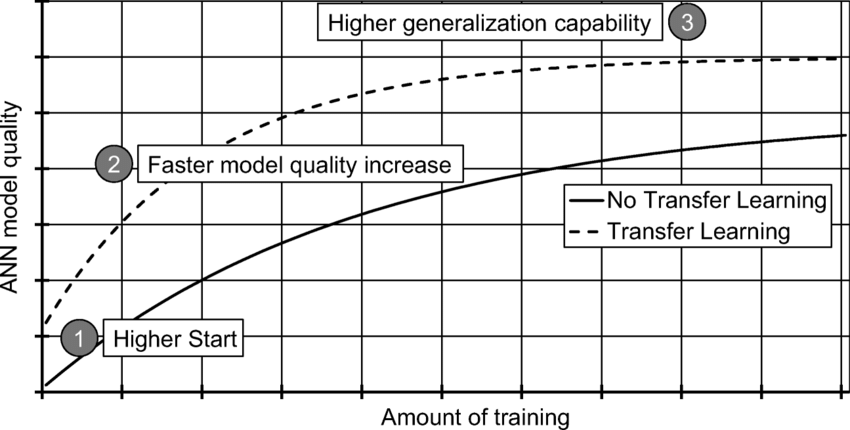
\includegraphics[scale = 0.5]{Images/Theoretical basis/Possible-advantages-of-transfer-learning.png}
\caption{Lợi ích của Transfer Learning}
\end{figure}


\begin{itemize}
    \item Cải thiện hiệu suất của mô hình, đặc biệt là khi dữ liệu huấn luyện hạn chế.
    \item Giảm thời gian huấn luyện và tài nguyên tính toán.
    \item Nâng cao khả năng khái quát hóa của mô hình.
\end{itemize}

\textbf{Bất lợi:}

\begin{itemize}
    \item Có thể xảy ra hiện tượng "negative transfer" nếu miền nguồn và miền đích quá khác biệt.
    \item Khó khăn trong việc lựa chọn mô hình tiền huấn luyện phù hợp.
\end{itemize}
\subsection{Giới thiệu về Self-Attention}

Self-attention là một cơ chế trong học sâu cho phép mô hình tập trung vào các phần khác nhau của dữ liệu đầu vào khi xử lý nó. Nó đã trở thành một thành phần quan trọng trong nhiều kiến trúc mạng nơ-ron hiện đại, đặc biệt là trong lĩnh vực xử lý ngôn ngữ tự nhiên.

\subsubsection{Cơ chế hoạt động của Self-Attention}

Self-attention hoạt động bằng cách tính toán mối quan hệ giữa các phần tử khác nhau trong một chuỗi. Mỗi phần tử được biểu diễn bằng một vector, và self-attention tính toán "attention weights" (trọng số chú ý) để xác định mức độ quan trọng của mỗi phần tử đối với các phần tử khác. Các trọng số này sau đó được sử dụng để tạo ra một biểu diễn mới cho mỗi phần tử, kết hợp thông tin từ các phần tử liên quan.


 \begin{figure}[H]
    \centering
    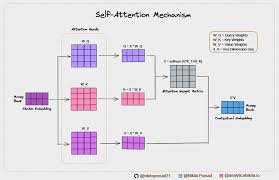
\includegraphics[scale = 1]{Images/Theoretical basis/self-attention.jpg}
\caption{Self Attention}
\end{figure}

\subsubsection{Các loại Self-Attention thường gặp}

Có nhiều biến thể của self-attention, mỗi biến thể có những đặc điểm và ứng dụng riêng:

\begin{itemize}
    \item \textbf{Scaled Dot-Product Attention:} Đây là biến thể phổ biến nhất, được sử dụng trong Transformer. Nó tính toán attention weights dựa trên tích vô hướng của các vector biểu diễn.
    \item \textbf{Multi-Head Attention:}  Biến thể này sử dụng nhiều "head" attention song song, mỗi head tập trung vào các khía cạnh khác nhau của dữ liệu.
    \item \textbf{Additive Attention:} Biến thể này sử dụng một mạng nơ-ron để tính toán attention weights.
\end{itemize}

\subsubsection{Ứng dụng của Self-Attention}

Self-attention đã được ứng dụng rộng rãi trong nhiều lĩnh vực:

\begin{itemize}
    \item \textbf{Xử lý ngôn ngữ tự nhiên:} 
    \begin{itemize}
        \item Dịch máy
        \item Tóm tắt văn bản
        \item Phân tích cảm xúc
        \item Hỏi đáp
    \end{itemize}
    \item \textbf{Thị giác máy tính:}
    \begin{itemize}
        \item Phân loại ảnh
        \item Nhận dạng đối tượng
    \end{itemize}
    \item \textbf{Các lĩnh vực khác:}
    \begin{itemize}
        \item Sinh học
        \item Âm nhạc
    \end{itemize}
\end{itemize}

\subsubsection{Lợi ích của Self-Attention}

\begin{itemize}
    \item \textbf{Nắm bắt được các phụ thuộc dài hạn:} Self-attention có thể nắm bắt được mối quan hệ giữa các phần tử cách xa nhau trong chuỗi, điều mà các mô hình RNN truyền thống gặp khó khăn.
    \item \textbf{Tính toán song song hiệu quả:} Self-attention có thể được tính toán song song, giúp tăng tốc độ huấn luyện và suy luận.
    \item \textbf{Khả năng diễn giải tốt:} Attention weights cung cấp thông tin về các phần tử quan trọng trong chuỗi, giúp hiểu rõ hơn cách mô hình đưa ra quyết định.
\end{itemize}

\subsection{Nội suy tuyến tính (Linear Interpolation)}

\begin{figure}[H]
    \centering
    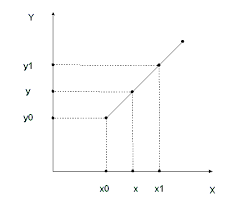
\includegraphics[scale = 1]{Images/Theoretical basis/linear_interpolation.png}
    \caption{Nội suy tuyến tính}    
\end{figure}

Nội suy tuyến tính là một phương pháp ước tính giá trị của một hàm số tại một điểm chưa biết, dựa trên giá trị của hàm số tại hai điểm đã biết. 

Giả sử ta có hai điểm dữ liệu $(x_1, y_1)$ và $(x_2, y_2)$, và ta muốn ước tính giá trị của hàm số $y = f(x)$ tại điểm $x$ nằm giữa $x_1$ và $x_2$. Nội suy tuyến tính giả định rằng hàm số $f(x)$ là một đường thẳng giữa hai điểm đã biết. 

Công thức nội suy tuyến tính được cho bởi:

$y = y_1 + \frac{(x - x_1)}{(x_2 - x_1)}(y_2 - y_1)$

Trong lĩnh vực học máy, nội suy tuyến tính thường được sử dụng để tạo ra các điểm dữ liệu mới từ tập dữ liệu hiện có. Ví dụ, trong bài toán xử lý ảnh, nội suy tuyến tính có thể được sử dụng để phóng to hoặc thu nhỏ ảnh. 

\subsubsection{Lợi ích của nội suy tuyến tính}
\begin{itemize}
    \item \textbf{Đơn giản:} Nội suy tuyến tính là một phương pháp đơn giản và dễ hiểu để ước lượng giá trị của một hàm số tại một điểm chưa biết.
\end{itemize}

\subsubsection{Hạn chế của nội suy tuyến tính}
\begin{itemize}
    \item \textbf{Giả định tuyến tính:} Nội suy tuyến tính giả định rằng hàm số là một đường thẳng giữa hai điểm đã biết, điều này có thể không phản ánh đúng mối quan hệ giữa các điểm dữ liệu.
\end{itemize}

\subsection{Generative Adversarial Networks (GANs)}

Generative Adversarial Networks (GANs) là một lớp mô hình học sâu mạnh mẽ được sử dụng để tạo ra dữ liệu mới, giống với dữ liệu huấn luyện. GANs bao gồm hai thành phần chính: generator và discriminator, hoạt động theo một cách đối kháng - generator cố gắng sinh dữ liệu sao cho giống với dữ liệu thật nhất, discriminator cố gắng phân biệt giữa dữ liệu sinh ra và dữ liệu thật cho đến khi discrimator không thể phân biệt được nữa.

 \begin{figure}[H]
    \centering
    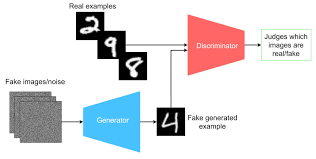
\includegraphics[scale = 0.8]{Images/Theoretical basis/GAN.png}
\caption{Generative Adversarial Networks (GANs)}
\end{figure}

\subsubsection{Kiến trúc và hoạt động của GANs}

\begin{itemize}
    \item \textbf{Generator:} Mạng nơ-ron này nhận vào một vector nhiễu ngẫu nhiên và cố gắng tạo ra dữ liệu giả mạo giống với dữ liệu thật.
    \item \textbf{Discriminator:} Mạng nơ-ron này nhận vào dữ liệu (thật hoặc giả mạo) và cố gắng phân biệt giữa chúng.
\end{itemize}
Hai mạng này được huấn luyện đồng thời: generator cố gắng đánh lừa discriminator, trong khi discriminator cố gắng không bị đánh lừa. Quá trình huấn luyện này tạo ra một vòng lặp phản hồi, trong đó cả hai mạng đều cải thiện theo thời gian.

\subsubsection{Các biến thể của GANs}

Có nhiều biến thể của GANs, mỗi biến thể có những đặc điểm và ứng dụng riêng:

\begin{itemize}
    \item \textbf{Deep Convolutional GANs (DCGANs):} Sử dụng mạng nơ-ron tích chập để tạo ra hình ảnh chất lượng cao.
    \item \textbf{Conditional GANs (cGANs):} Cho phép điều khiển quá trình tạo dữ liệu bằng cách cung cấp thông tin bổ sung (như nhãn lớp).
    \item \textbf{CycleGANs:} Cho phép chuyển đổi dữ liệu từ miền này sang miền khác (ví dụ: chuyển đổi ảnh từ mùa hè sang mùa đông).
    \item \textbf{Progressive Growing of GANs (PGGANs):}  Tạo ra hình ảnh có độ phân giải cao bằng cách tăng dần kích thước của mạng generator và discriminator.
    \item \textbf{StyleGAN:} Tạo ra hình ảnh chân thực với khả năng kiểm soát các thuộc tính tinh tế.
    \item \textbf{TimeGAN:} Tạo ra dữ liễu chuỗi thời gian mẫu từ tập dữ liệu đầu vào cho sẵn
\end{itemize}

\subsubsection{Ứng dụng của GANs}

GANs đã được ứng dụng trong nhiều lĩnh vực:

\begin{itemize}
    \item \textbf{Tạo hình ảnh:} Tạo ra hình ảnh chân thực của người, vật thể, cảnh quan,...
    \item \textbf{Tạo dữ liệu:} Tạo ra dữ liệu tổng hợp cho các tác vụ học máy khác.
    \item \textbf{Chỉnh sửa ảnh:}  Thay đổi các thuộc tính của ảnh (ví dụ: thêm nụ cười, thay đổi kiểu tóc).
    \item \textbf{Siêu phân giải ảnh:} Tăng độ phân giải của ảnh.
    \item \textbf{Phục hồi ảnh:} Khôi phục các phần bị thiếu hoặc bị hỏng của ảnh.
\end{itemize}

\subsubsection{Lợi ích và hạn chế của GANs}

\textbf{Lợi ích:}

\begin{itemize}
    \item Khả năng tạo ra dữ liệu mới, đa dạng và chân thực.
    \item Ứng dụng rộng rãi trong nhiều lĩnh vực.
\end{itemize}

\textbf{Hạn chế:}

\begin{itemize}
    \item Huấn luyện GANs có thể khó khăn và không ổn định.
    \item Đánh giá chất lượng của dữ liệu do GANs tạo ra có thể phức tạp.
\end{itemize}

\subsection{Giới thiệu về thư viện Tensorflow}
\indent TensorFlow là một thư viện mã nguồn mở được phát triển bởi Google, được sử dụng để xây dựng các mô hình học máy và mạng nơ-ron. TensorFlow sẽ giúp giải quyết các bài toán nhanh chóng và đơn giản hơn thông qua việc tạo các mô hình tính toán trong Machine Learning trên máy tính.
\begin{figure}[H]
    \centering
    
\includegraphics[width=\textwidth,height=\textheight,keepaspectratio]{Images/Theoretical basis/TensorFlow_logo.png}
    \caption{Thư viện Tensorflow}
    \label{fig:enter-label}
\end{figure}
\subsubsection{Nguyên lý hoạt động}
\indent Tensorflow là một thư viện tính toán số và biểu diễn dữ liệu bằng cấu trúc đồ thị (graph) để tạo và huấn luyện các mô hình học máy. Các đồ thị này bao gồm các nút (nodes) và các cạnh (edges) được sử dụng để biểu diễn các phép tính và dữ liệu tương ứng trong mô hình. Một cách tổng quát, quá trình huấn luyện mô hình học máy trong TensorFlow trải qua các bước sau:

\begin{itemize}
    \item \textbf{Xây dựng đồ thị tính toán:} Người dùng xác định cấu trúc đồ thị tính toán bằng cách khai báo các biến (variables) và các phép tính (operations) trong mô hình.
    \item \textbf{Định nghĩa hàm mất mát:} Hàm mất mát (loss function) được định nghĩa để đo lường sự khác biệt giữa đầu ra dự đoán của mô hình và giá trị thực tế.
    \item \textbf{Tối ưu hóa mô hình:} Quá trình tối ưu hóa được sử dụng để tìm ra các giá trị tham số tối ưu nhằm giảm thiểu hàm mất mát.
    \item \textbf{Huấn luyện mô hình:} Dữ liệu huấn luyện được đưa vào mô hình để huấn luyện và cập nhật các giá trị tham số.
    \item \textbf{Đánh giá mô hình:} Dữ liệu kiểm tra được sử dụng để đánh giá hiệu suất của mô hình.
    \item \textbf{Sử dụng mô hình:} Mô hình đã huấn luyện được sử dụng để dự đoán và phân loại các dữ liệu mới.
\end{itemize}
\begin{figure}[H]
    \centering
    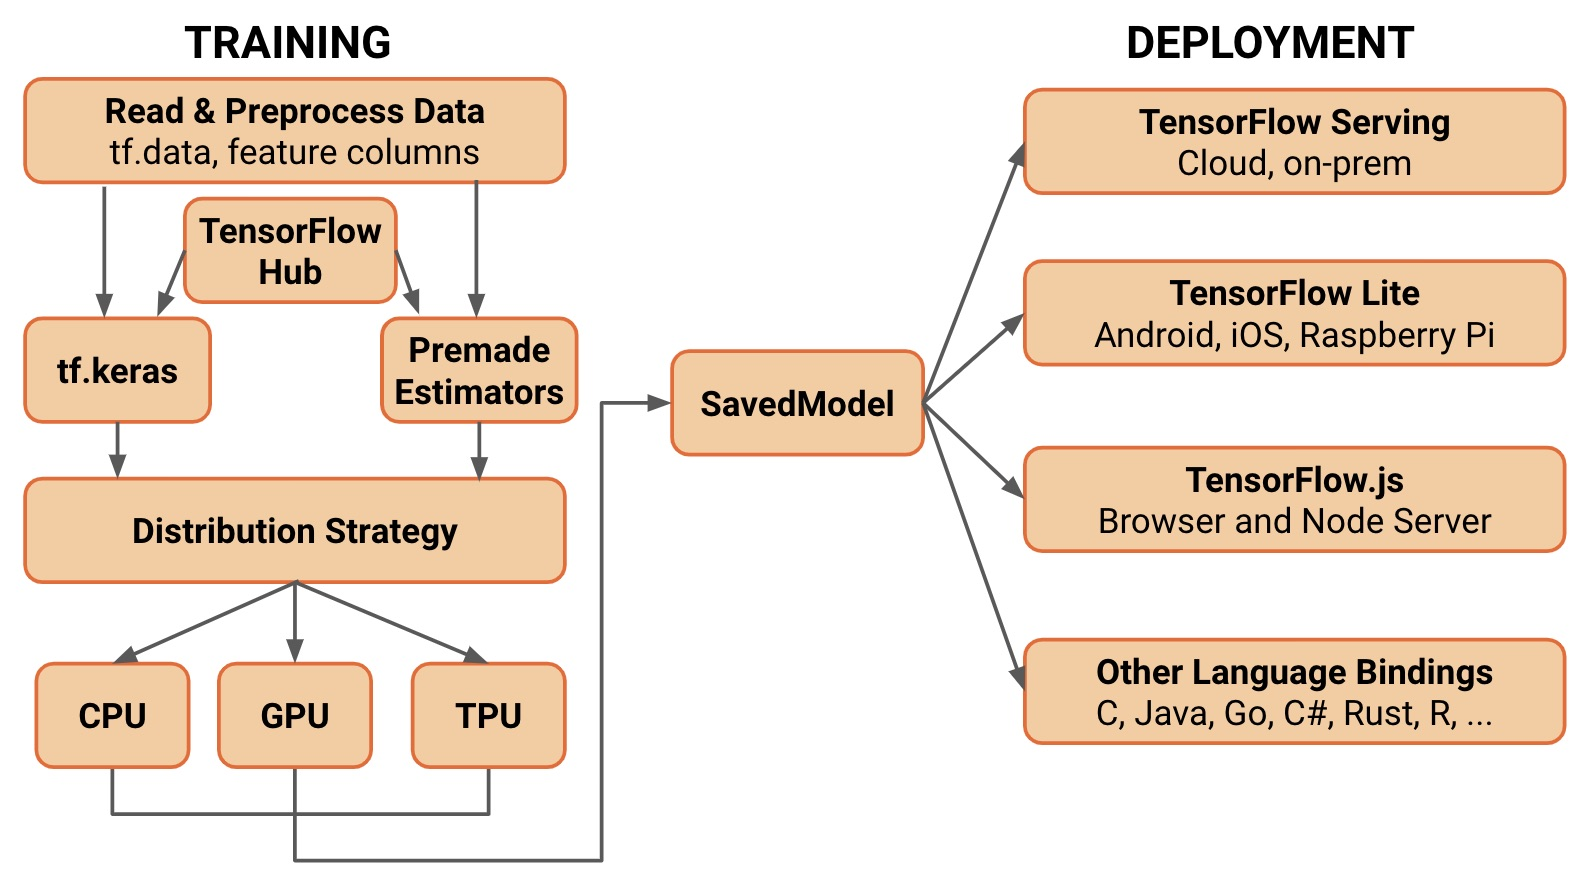
\includegraphics[width=\textwidth,height=\textheight,keepaspectratio]{Images/Theoretical basis/nguyen-li-hoat-dong-tensorflow.jpeg}
    \caption{Nguyên lý hoặc động của Tensorflow}
    \label{fig:enter-label}
\end{figure}


\subsubsection{Thuộc tính cơ bản trong Tensorflow}
\indent Về cơ bản thì các thuộc tính của TensorFlow bao gồm:
\begin{itemize}
    \item \textbf{Tensors:} Là đối tượng chính của TensorFlow, đại diện cho dữ liệu và kết quả tính toán. Tensors là một mảng đa chiều có các phần tử có cùng kiểu dữ liệu.
    
    \begin{figure}[H]
        \centering
        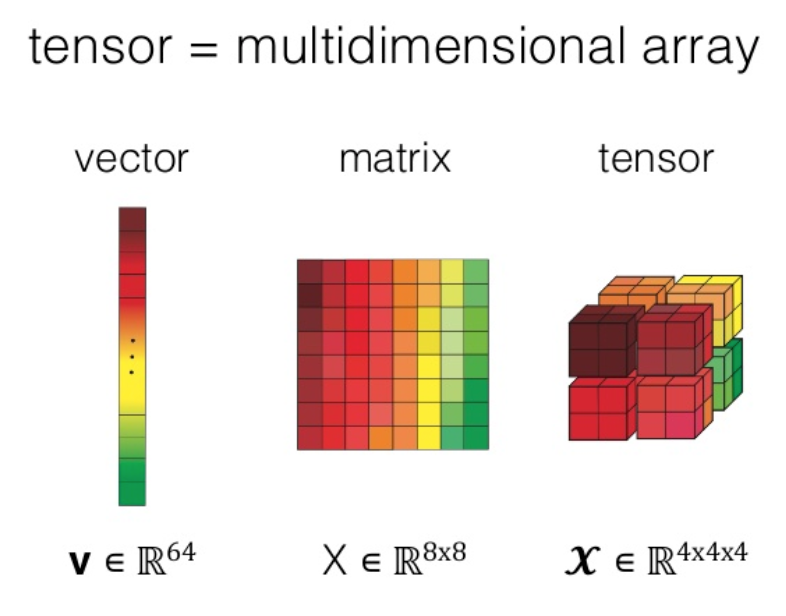
\includegraphics[width=\textwidth,height=\textheight,keepaspectratio]{Images/Theoretical basis/tensor.png}
        \caption{Hình ảnh minh họa của một tensor và so sánh với vector và ma trận.}
        \label{fig:enter-label}
    \end{figure}
    \item \textbf{Phép tính toán(Operations):} Là các hoạt động được thực hiện trên các tensors. Một số hoạt động cơ bản của TensorFlow bao gồm phép cộng, trừ, nhân và chia.
    \item \textbf{Biến(Variables):} Là các đối tượng được sử dụng để lưu trữ trạng thái thay đổi được trong quá trình huấn luyện mô hình. Variables có thể được khởi tạo với giá trị cố định hoặc giá trị ngẫu nhiên và có thể được cập nhật trong quá trình huấn luyện.

    \item \textbf{Đồ thị(Graphs):} Là các biểu đồ đại diện cho các phép tính và các kết nối giữa chúng. Graphs được sử dụng để mô tả cấu trúc của mô hình học máy và tạo ra các tính toán hiệu quả trên nhiều thiết bị tính toán.

    \item \textbf{Sessions:} Là một phiên làm việc TensorFlow, chứa tất cả các biến và phép tính cần thiết để thực hiện tính toán. Sessions được sử dụng để thực thi các tính toán trong TensorFlow.
    \begin{figure}[H]
        \centering
        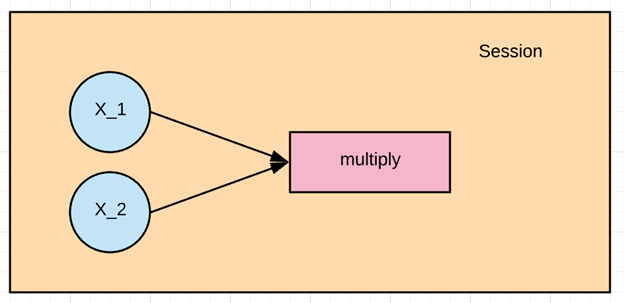
\includegraphics[width=\textwidth,height=\textheight,keepaspectratio]{Images/Theoretical basis/083018_0508_WhatisTenso2.png}
        \caption{Minh họa cho 1 graph, session, operation và variable.}
        \label{fig:enter-label}
    \end{figure}
    \item \textbf{Placeholders:} Là các đối tượng được sử dụng để đại diện cho các tensors được cung cấp vào mô hình trong quá trình huấn luyện hoặc kiểm tra. Placeholders được sử dụng để đảm bảo rằng dữ liệu đầu vào có thể được cung cấp cho mô hình.
\end{itemize}

Các thuộc tính này là những thành phần cơ bản của TensorFlow và cung cấp các công cụ cần thiết để xây dựng và huấn luyện các mô hình học máy hiệu quả.

\subsubsection{Ưu điểm của TensorFlow}
\indent TensorFlow cung cấp các công cụ hỗ trợ cho việc xây dựng, huấn luyện và triển khai các mô hình học máy một cách linh hoạt và hiệu quả trên nhiều nền tảng khác nhau. TensorFlow sở hữu nhiều ưu điểm vượt trội như sau:
\begin{itemize}
    \item Tính linh hoạt: TensorFlow không chỉ hỗ trợ một loạt các thuật toán học máy và học sâu, mà còn cho phép người dùng tạo ra các mô hình học máy tùy chỉnh của riêng họ.
    \item Khả năng mở rộng: TensorFlow có thể chạy trên nhiều nền tảng khác nhau, từ máy tính cá nhân đến các máy chủ lớn, và thậm chí là các thiết bị di động.
    \item Hiệu suất cao: TensorFlow tận dụng tối đa sức mạnh của phần cứng bằng cách sử dụng đa luồng và tính toán song song.
    \item Hỗ trợ cộng đồng: Với một cộng đồng người dùng lớn và tích cực, TensorFlow cung cấp nhiều tài liệu học tập và hỗ trợ từ cộng đồng.
\end{itemize}

\subsection{Giới thiệu về Arduino LilyPad}
\indent LilyPad Arduino là một dạng bo mạch Arduino được thiết kế đặc biệt cho các thiết bị điện tử mặc được và e-textiles.  mạch có thể được may vào vải và gắn với các nguồn điện, cảm biến và actuator bằng chỉ dẫn điện.
\begin{figure}[H]
    \centering
    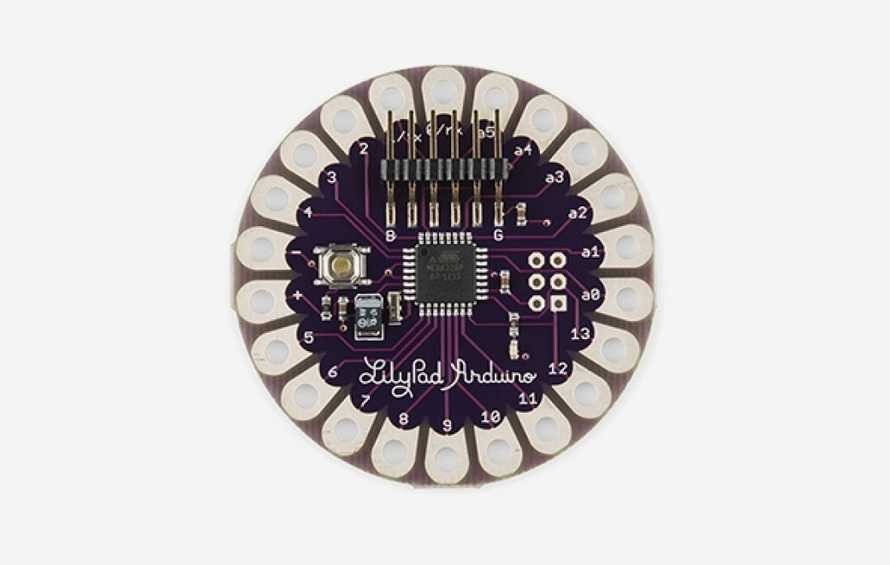
\includegraphics[width=\textwidth,height=\textheight,keepaspectratio]{Images/Theoretical basis/lilypad_main.jpg}
    \caption{Board mạch Arduino Lilypad}
    \label{fig:enter-label}
\end{figure}
\indent Arduino Lilypad được thiết kế và phát triển bởi Leah Buechley và SparkFun Electronics. Board mạch được thiết kế dựa trên chip điều khiển ATmega168V hoặc ATmega328V. Dưới đây là thông số kỹ thuật của  Arduino LilyPad:

\begin{longtblr}[
  caption = {Thông số kỹ thuật của Arduino Lilypad},
]{
  width = \linewidth,
  colspec = {Q[404]Q[521]},
  hlines,
  vlines,
}
Vi điều khiển          & ATmega168 hoặc ATmega328V \\
Điện áp hoạt động      & 2.7-5.5 V                                                                                 \\
Điện áp đầu vào        & 2.7-5.5 V                                                                                 \\
Số chân I/O            & 14                                                                                        \\
Số kênh PWM            & 6                                                                                         \\
Số kênh đầu vào Analog & 6                                                                                         \\
Dòng điện mỗi chân     & 40mA                                                                                      \\
Bộ nhớ Flash           & 16 KB                                                                                     \\
SRAM                   & 1 KB                                                                                      \\
EEPROM                 & 512 bytes                                                                                 \\
Tần số xung            & 8 MHz                                                                                     
\end{longtblr}



\indent Một số ứng dụng của Arduino Lilypad:
\begin{itemize}
    \item \textbf{Quần áo thông minh:} Lilypad có thể được may vào trang phục kết hợp với các cảm biến khác tạo ra một bộ trang phục thông minh với các chức năng theo dõi thông số cơ thể.
    \item \textbf{Thiết bị đeo tay thông minh:} Có thể dùng Lilypad như như một đồng hồ đeo tay thông minh, găng tay thông minh để theo dõi cử chỉ bàn tay, hoặc cử chỉ của cơ thể.
\end{itemize}



\subsection{Giới thiệu về cảm biến uốn cong(Flex sensor)}


\subsubsection{Tổng quan} 

\indent Cảm biến uốn cong (flex sensor) thực chất là một biến trở có khả năng thay đổi điện trở khi được uốn cong. Vì điện trở biến thiên tỷ lệ thuận trực tiếp với độ uốn cong, nên nó thường được gọi là Potentiometer Uốn Cong.

\indent Cảm biến uốn cong thường có hai kích thước phổ biến: 2.2 inch (5.588cm) và 4.5 inch (11.43cm).

\begin{figure}[H]
    \centering
    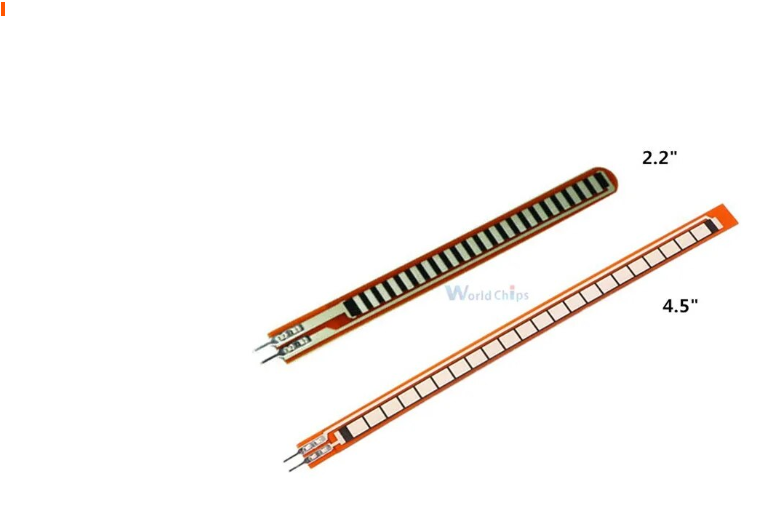
\includegraphics[width=9cm]{Images/Theoretical basis/flex sensor.png}
\caption{Flex sensor}
\end{figure}

\subsubsection{Nguyên lý hoạt động}

\begin{enumerate}[-]
    \item Mực dẫn trên cảm biến chính là một loại trở kháng. 
    \begin{itemize}
        \item Khi cảm biến thẳng, trở kháng này khoảng 25k.
        \item Khi cảm biến được uốn cong, lớp mực dẫn bị căng, dẫn đến giảm diện tích tiết diện (hãy tưởng tượng như việc căng một sợi dây cao su) và tăng trở kháng. Ở góc uốn cong 90°, trở kháng này khoảng 100K.
        \item Khi cảm biến được thẳng lại, trở kháng trở về giá trị ban đầu.
    \end{itemize}
    \item  Bằng cách đo trở kháng, ta có thể xác định được mức độ uốn cong của cảm biến.
\end{enumerate}

\begin{figure}[H]
    \centering
    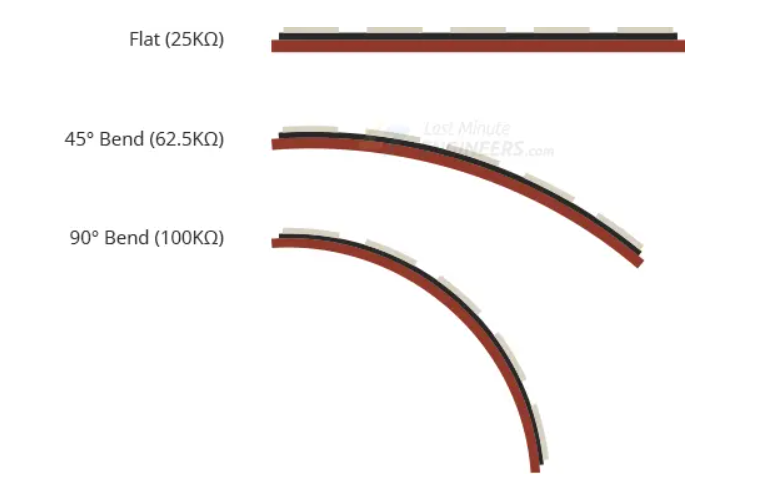
\includegraphics[width=11cm]{Images/Theoretical basis/flex sensor 1.png}
\caption{Hình dạng uốn cong của flex sensor}
\end{figure}

\subsubsection{Đọc giá trị}

\indent Cách đơn giản nhất để đọc cảm biến uốn cong (Flex Sensor) là kết hợp với một trở kháng tĩnh để tạo thành một bộ chia điện áp, từ đó tạo ra một điện áp biến đổi có thể đọc được bởi bộ chuyển đổi tương tự sang số của vi điều khiển.

\begin{figure}[H]
    \centering
    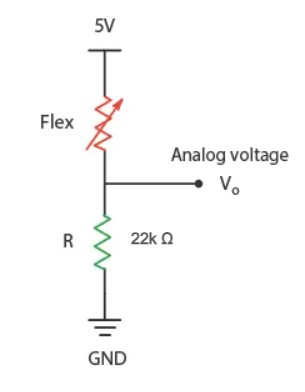
\includegraphics[width=5cm]{Images/Theoretical basis/flex sensor 2.jpg}
\caption{Sơ đồ nối dây của flex sensor}
\end{figure}

\indent Lưu ý rằng điện áp đầu ra mà bạn đo là mức giảm điện áp qua trở kháng kéo xuống, không phải là giảm điện áp qua cảm biến uốn cong (Flex Sensor).

\indent Chúng ta có thể sử dụng công thức sau để tính toán điện áp đầu ra (Vo).
\[ V_0 = \frac{V_{cc} \cdot R}{R + R_{\text{flex}}} \]

\indent Trong trường hợp này, điện áp đầu ra giảm khi bán kính uốn cong tăng lên.
\subsection{Giới thiệu về cảm biến con quay gia tốc}
\indent Cảm biến gia tốc hoạt động dựa trên nguyên lý của lực quán tính, thường thông qua cấu trúc vi cơ điện tử (MEMS). Bên trong cảm biến, có một khối lượng nhỏ gọi là vi khối lượng, được gắn vào một khung bằng các lò xo siêu nhỏ. Khi cảm biến trải qua gia tốc, vi khối lượng này sẽ dịch chuyển do lực quán tính. Sự dịch chuyển này được chuyển đổi thành tín hiệu điện bằng cách sử dụng các phương pháp như cảm ứng điện dung, hiệu ứng piezoelectric hoặc cầu Wheatstone.\\
\indent Nhờ vào cấu trúc và nguyên lý hoạt động tinh vi, cảm biến gia tốc có thể đo lường chính xác gia tốc theo nhiều trục, thường là ba trục (x, y, z), giúp cung cấp thông tin chi tiết về chuyển động và vị trí của vật thể trong không gian.
\subsubsection{Nguyên lý hoạt động}
\subsubsubsection{Sử dụng hiệu ứng Piezoelectric}
\indent Hiệu ứng Piezoelectric là hiện tượng mà một số vật liệu nhất định có khả năng tạo ra điện tích khi chịu áp lực cơ học. Từ “Piezoelectric” bắt nguồn từ từ tiếng Hy Lạp “piezein”, có nghĩa là “ấn hoặc nén”, mô tả chính xác quá trình tạo ra điện năng thông qua áp lực.

\indent Hiệu ứng này xảy ra ở mức độ vi mô, khi áp dụng một lực cơ học dẫn đến sự di chuyển của các điện tích dương và âm trong cấu trúc tinh thể của vật liệu. Sự dịch chuyển này tạo ra một cực điện và hình thành một điên áp đi qua vật liệu.

\indent Hiệu ứng Piezoelectric là một quá trình có thể đảo ngược: vật liệu thể hiện hiệu ứng piezoelectric cũng sẽ bị biến dạng cơ học nếu đặt một điện áp đi qua nó.

Ví dụ, các tinh thể titanate zirconate chì sẽ tạo ra dòng điện Piezoelectric khi cấu trúc tĩnh của chúng bị biến dạng khoảng 0,1\% so với kích thước gốc. Ngược lại, những tinh thể giống như vậy sẽ thay đổi khoảng 0,1\% kích thước tĩnh của chúng khi áp dụng một điện trường bên ngoài.

\indent Hiệu ứng Piezoelectric đã được khai thác trong nhiều ứng dụng hữu ích, bao gồm sản xuất và phát hiện âm thanh, in phun piezoelectric, tạo ra điện năng điện áp cao, như một bộ tạo xung trong các thiết bị điện tử, trong microbalances, để điều khiển một đầu phun siêu âm, và trong việc tập trung siêu mịn của các bộ phận quang học.
\begin{figure}[H]
    \centering
    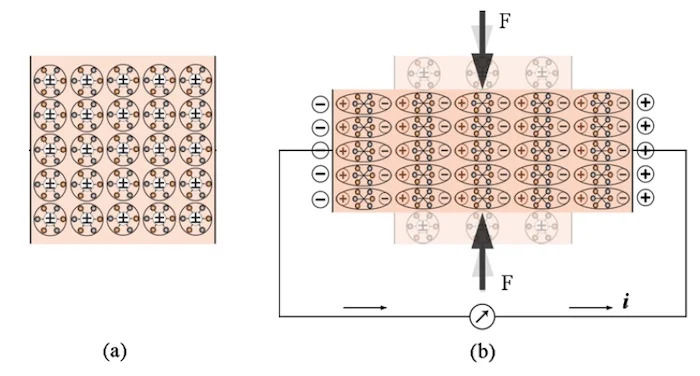
\includegraphics[width=\textwidth,height=\textheight,keepaspectratio]{Images/Theoretical basis/intro_piezo_accelerometers_figure_1.jpeg}
    \caption{Hiệu ứng Piezoelectric}
    \label{fig:pio_prin}
\end{figure}
\indent Cấu trúc của cảm biến gia tốc bao gồm một phần tử piezoelectric để kết nối một lượng khối lượng cố định với thân cảm biến. Khi khung cảm biến tăng tốc do lực bên ngoài, khối lượng tham chiếu có xu hướng giữ nguyên vị trí do quán tính và làm biến dạng nhẹ phần tử piezoelectric.
\indent Nếu nối hai điện cực với nhau thông qua một sợi dây như mô tả trong \ref{fig:pio_prin}, thì các electron tự do trong dây dẫn sẽ chảy về phía điện cực tích điện dương và tạo ra một dòng điện. Dòng điện này tích tụ các electron tự do trên điện cực dương và tạo ra một điện trường ngược hướng với trường ban đầu được tạo ra bởi hiệu ứng Piezoelectric.

\indent Hiệu ứng này giải thích tại sao dòng điện do lực tĩnh tạo ra chỉ có thể tồn tại trong một khoảng thời gian ngắn. Dòng điện tiếp tục cho đến khi điện trường do sự tích tụ của các electron tự do triệt tiêu trường khỏi hiệu ứng Piezoelectric.
\begin{figure}[H]
    \centering
    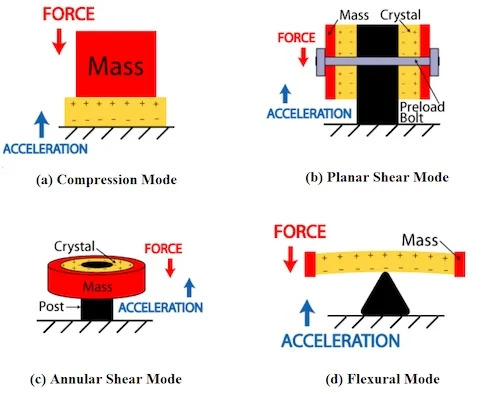
\includegraphics[width=\textwidth,height=\textheight,keepaspectratio]{Images/Theoretical basis/intro_piezo_accelerometers_figure_2.jpeg}
    \caption{Các kiểu thiết kế cơ học của cảm biến gia tốc}
    \label{fig:piozDesin}
\end{figure}
\indent Các kiểu thiết kế cơ học phổ biến của cảm biến gia tốc sử dụng hiệu ứng Piezoelectric:
\begin{itemize}
    \item \textbf{Thiết kế theo chế độ nén:} THiết kế này rất đơn giản, chỉ bao gồm một bản thiết bị có hiệu ứng Piezoelectric và một khối lượng tham chiếu. Khi xảy ra gia tốc, lực quán tính sẽ làm cho khối lượng tham chiếu ép chặt vào tấm vật liệu áp điện từ đó tạo ra dòng điện.
    \item \textbf{Thiết theo chế độ trượt:} Gồm hai loại là trượt trên một tấm phẳng hoặc thiết kế trượt trên một khối hình nhẫn. Về cơ bản thì hai kiểu thiết kế này có cùng ngueyen lý hoạt động. Tinh thể được kẹp giữa trụ trung tâm và khối lượng thâm chiếu bên ngoài. Khối lượng càng nhiều thì lực trượt tác dụng lên tinh thể càng lớn đối với một gia tốc nhất định. Cấu trúc này giúp gia tốc kế cứng chắc, tạo ra dải tần số cao và do tinh thể không tiếp xúc trực tiếp với  cảm biến nên các hiệu ứng biến dạng và chuyển tiếp nhiệt được giảm thiểu.
    \item \textbf{Thiết kế theo chế độ uốn:} thiết kế này sử dụng các tấm tinh thể có hình chữ nhật hoặc hình đĩa. Sự uốn cong của tinh thể có thể xảy ra do khối lượng của chính tinh thể đối lập với gia tốc hoặc để tăng cường sự uốn cong, trọng lượng bổ sung có thể được kẹp hoặc liên kết với tinh thể. Gia tốc kế ở chế độ uốn ít cứng hơn khi so sánh với thiết kế nén hoặc trượt, cung cấp cho chúng dải tần số giới hạn. Ngoài ra, do tinh thể phải chịu mức độ căng áp lực cao nên chúng dễ bị hỏng hơn các loại khác nếu bị sốc hoặc rung quá mức.
\end{itemize}


\subsubsubsection{Sử dụng phương pháp điện dung}
\indent Cấu trúc lò xo-khối nặng-giảm xóc: Cấu trúc này chuyển đổi gia tốc của khung cảm biến thành sự dịch chuyển của khối nặng chứng minh, và phương pháp cảm biến điện dung được áp dụng để chuyển đổi sự dịch chuyển này thành tín hiệu điện tử tỷ lệ với gia tốc được áp dụng.
\begin{figure}[H]
    \centering
    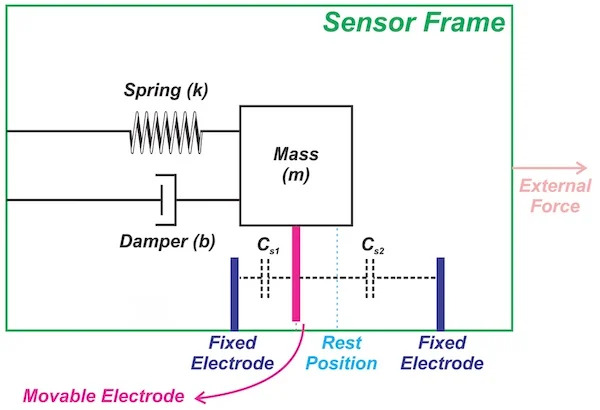
\includegraphics[width=\textwidth,height=\textheight,keepaspectratio]{Images/Theoretical basis/168_Introduction_to_Capacitive_Acceleration_Sensors_Figure_3.jpeg}
    \caption{Cấu trúc của một cảm biến gia tốc sử dụng phương pháp điện dung}
    \label{fig:capacitive_sensor}
\end{figure}
\indent Phương pháp cảm biến điện dung: Có hai bản điện cực được gắn cố định vào khung cảm biến cùng với một điện cực di động được kết nối với khối lượng tham chiếu. Thiết kế này hình thành hai tụ điện biến thiên C1 và C2, như được hiển thị trong hình \ref{fig:capacitive_sensor}.

\indent Khi khối lượng tham chiếu di chuyển theo một hướng dưới ảnh hưởng của gia tốc, điện dung giữa điện cực di động và một trong hai điện cực cố định tăng lên trong khi điện dung của tụ điện kia giảm xuống. Bằng cách đo đạc sự thay đổi điện dung của hai tụ điện trên, và kết hợp với khối lượng tham chiếu có sẳn ta có thể tính toán được gia tốc đầu vào.

\subsubsection{Giới thiệu về module cảm biến ITG 3200}
\begin{figure}[H]
    \centering
    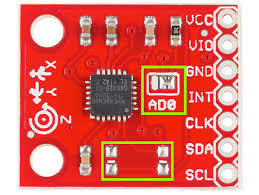
\includegraphics[width=\textwidth,height=\textheight,keepaspectratio]{Images/Theoretical basis/ITG3200.jpg}
    \caption{Cảm biến gia tốc góc ITG 3200}
    \label{fig:capacitive_sensor}
\end{figure}
Cảm biến gia tốc góc ITG-3200 là một loại cảm biến gia tốc góc (gyroscope) được sản xuất bởi InvenSense. Đây là một cảm biến quan trọng được sử dụng rộng rãi trong các ứng dụng đo lường và điều khiển chuyển động. Dưới đây là một số đặc điểm chính và thông tin cơ bản về ITG-3200:

Đặc điểm chính
\begin{itemize}
\item \textbf{Trục đo}: ITG-3200 là cảm biến 3 trục, có khả năng đo gia tốc góc trên ba trục X, Y và Z.
\item \textbf{Dải đo} (Range): Cảm biến này có thể đo gia tốc góc lên đến ±2000 độ/giây, phù hợp cho nhiều ứng dụng khác nhau từ điều khiển bay của máy bay không người lái đến các thiết bị chơi game.
 \item \textbf{Tốc độ lấy mẫu} (Sampling Rate): Cảm biến hỗ trợ tốc độ lấy mẫu lên đến 8 kHz, giúp thu thập dữ liệu nhanh và chính xác.
 \item \textbf{Giao tiếp}: ITG-3200 sử dụng giao tiếp I2C (Inter-Integrated Circuit), giúp dễ dàng kết nối với các vi điều khiển và các hệ thống nhúng khác.
\item \textbf{Nguồn điện}: Cảm biến hoạt động với điện áp từ 2.1V đến 3.6V, và thường được cấp điện áp 3.3V.
\item \textbf{Bộ lọc tích hợp}: Cảm biến này có tích hợp bộ lọc kỹ thuật số để giảm nhiễu và cải thiện độ chính xác của dữ liệu.
\end{itemize}
\subsection{Giới thiệu về module bluetooth HC05}
\begin{figure}[H]
    \centering
    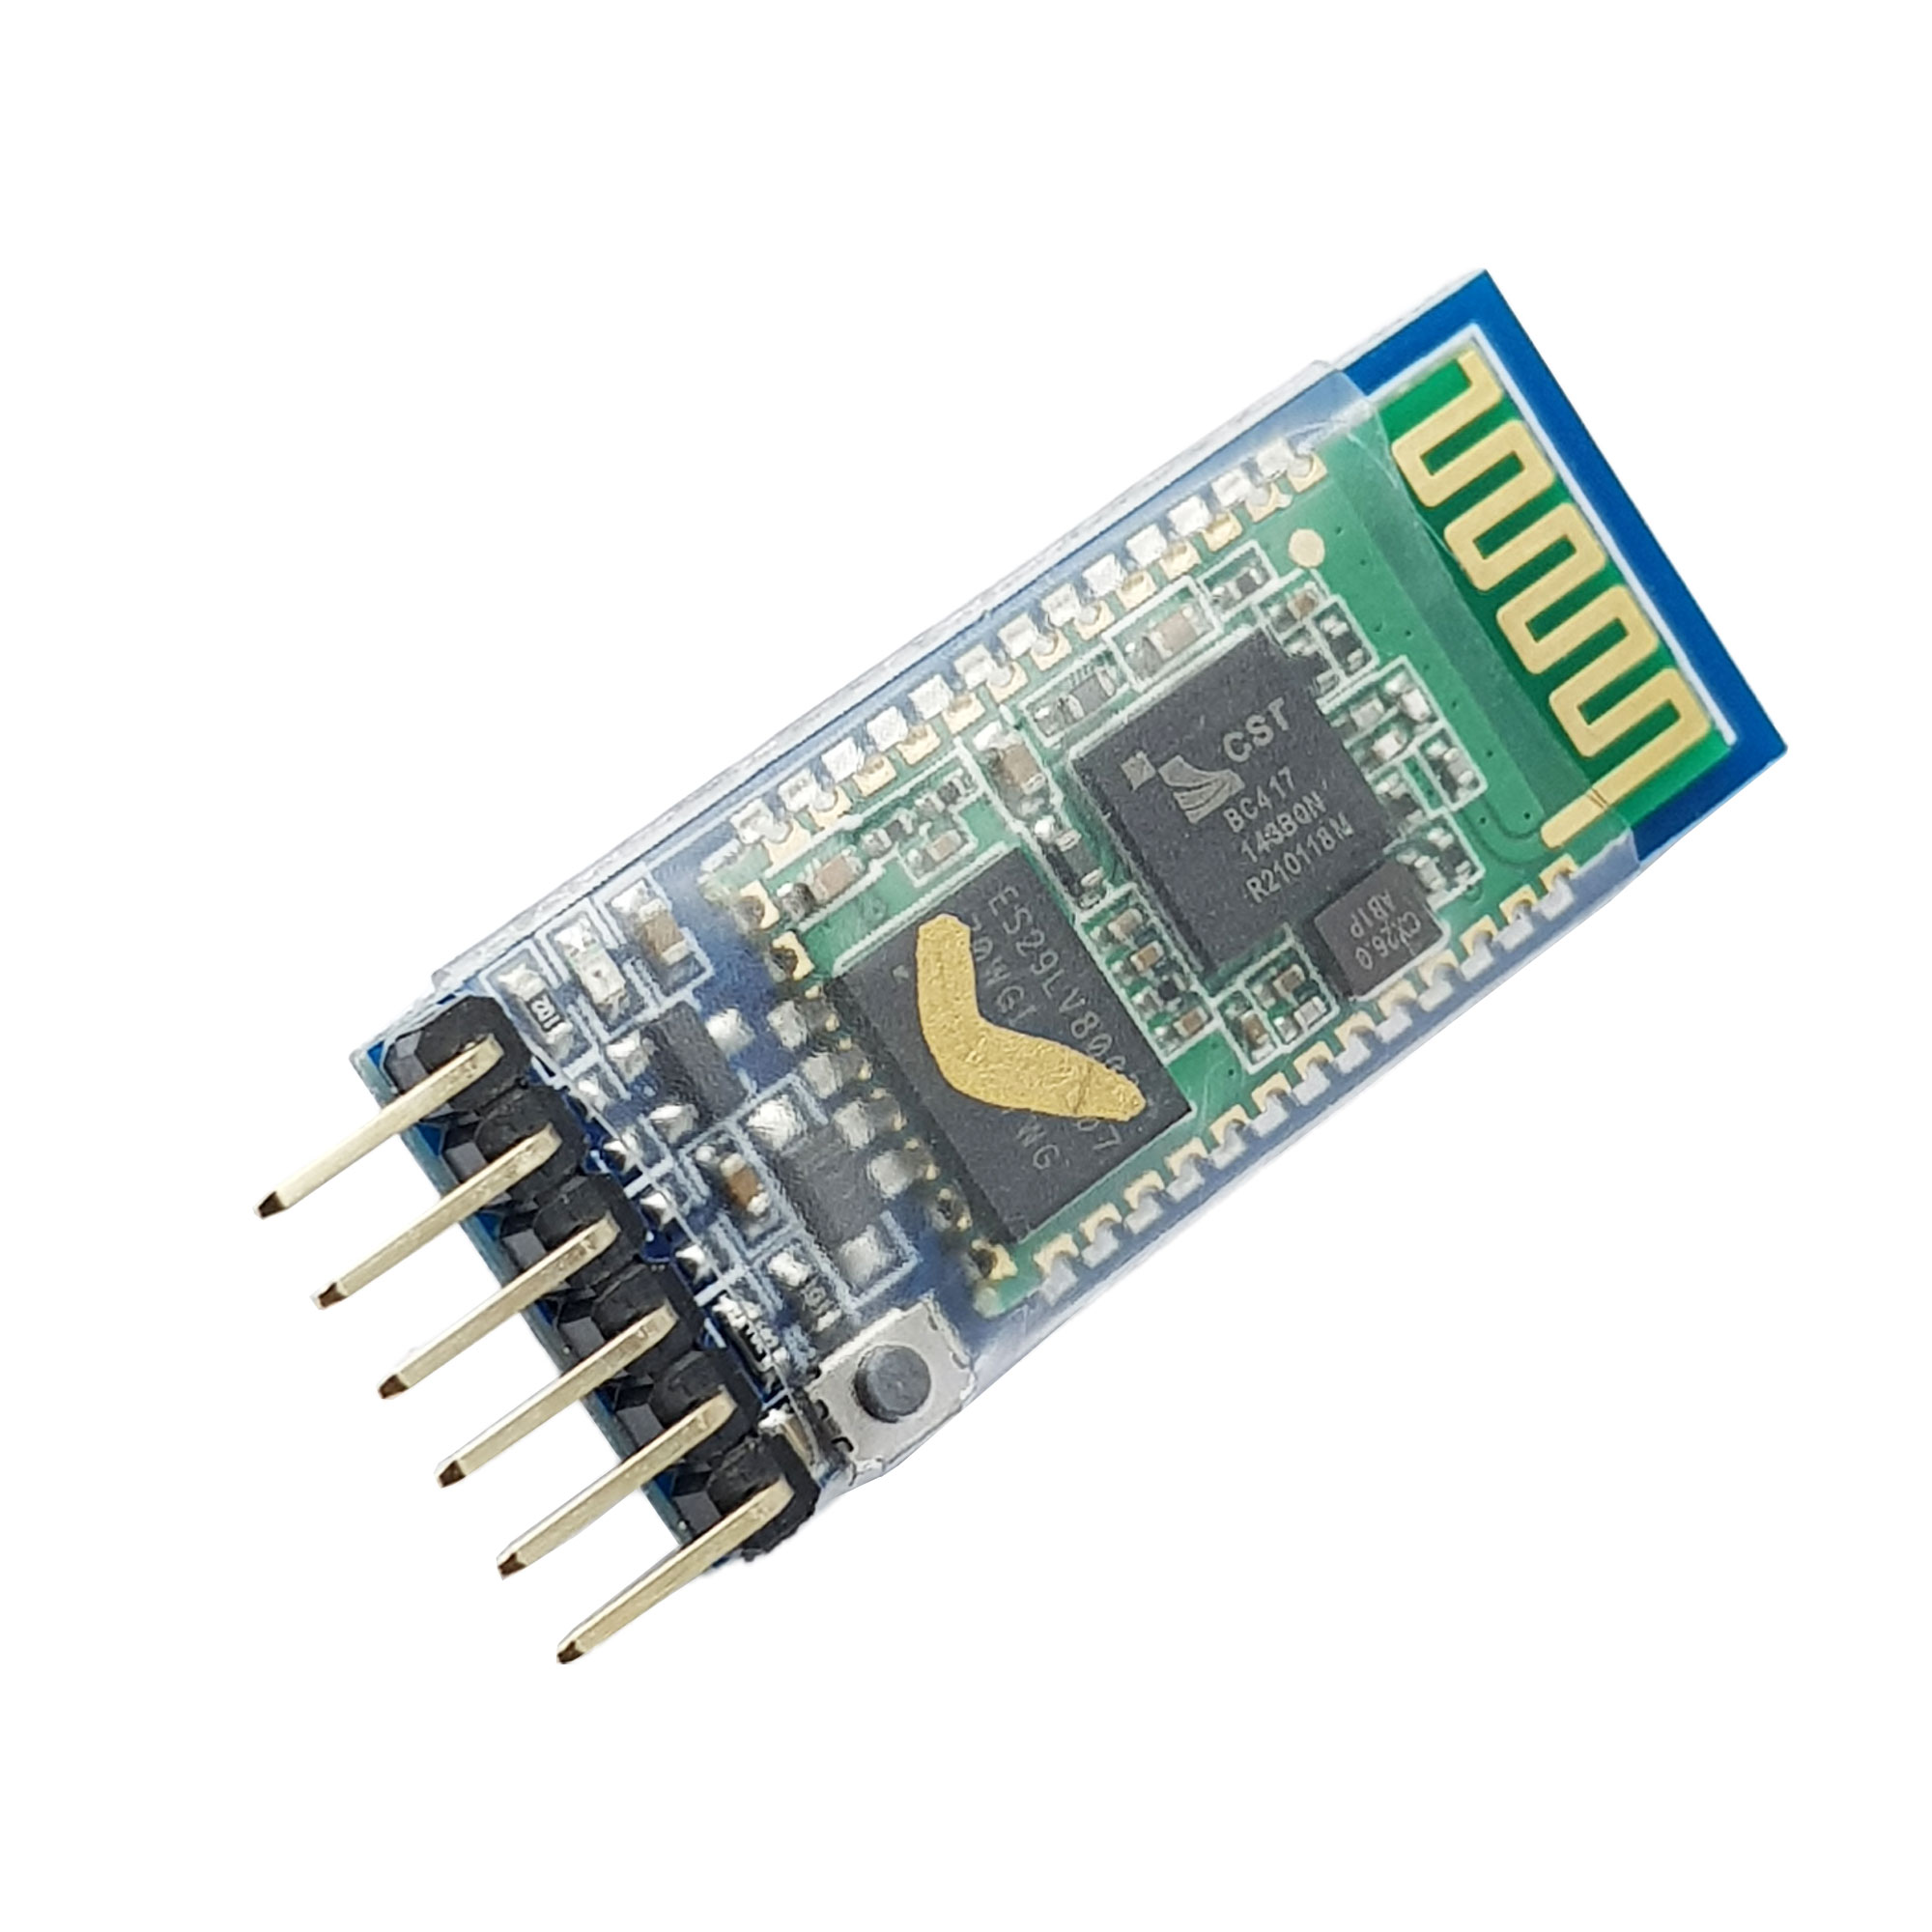
\includegraphics[width=\textwidth,height=\textheight,keepaspectratio]{Images/Theoretical basis/hc05.jpg}
    \caption{module bluetooth HC-05}
    \label{fig:capacitive_sensor}
\end{figure}

HC-05 là thiết bị Bluetooth tốt nhất sử dụng giao thức truyền thông UART. HC-05 Bluetooth có nhiều tính năng khác biệt so với tất cả các thiết bị Bluetooth khác vì có nhiều chân và chức năng.

Module thường sử dụng giao tiếp nối tiếp UART với các chân TX và RX ở tốc độ baund 9600. Có giao tiếp truyền dữ liệu hai chiều và có thể hoạt động như một slave và master.

Module Bluetooth chỉ cung cấp khả năng giao tiếp trong khoảng cách ngắn do có giới hạn, hầu hết do đảm bảo tốc độ và tính bảo mật của nó.

Mô tả sơ đồ chân
\begin{itemize}
    

\item \textbf{Chân VCC} Giống như mọi thiết bị khác, HC05 Modules cũng phụ thuộc vào nguồn điện để hoạt động và chân VCC cấp nguồn điện từ bên ngoài.

\item \textbf{Chân GND} Chân nối đất module.

\item \textbf{Chân TX} Chân truyền dữ liệu giao thức UART

\item \textbf{Chân RX} Chân nhận dữ liệu trong giao tiếp UART.

\item \textbf{Chân State} Báo trạng thái kết nối của Bluetooth.

\item \textbf{Chân Enable/key C} là chân thay đổi chế độ giữa chế độ dữ liệu và chế độ dòng lệnh bằng cách cấp tín hiệu bên ngoài. Cấp logic cao sẽ chuyển sang chế độ dòng lệnh và trạng thái logic thấp sẽ chuyển sang chế độ dữ liệu. Chế độ thiết bị mặc định là chế độ dữ liệu.

\item \textbf{Nút button} Các chế độ dữ liệu và lệnh có thể thay đổi thông qua một nút nhấn có trên module.

\item \textbf{Đèn LED}: Đèn LED hiển thị trạng thái của Module HC-05.

\end{itemize}

\indent \textbf{Đặc tính Bluetooth HC-05 }
\begin{itemize}
\item Module Bluetooth HC-05 cung cấp hai giao tiếp trong khoảng cách ngắn hơn với tốc độ nhanh.
\item  Có chân enale cho phép chuyển đổi giữa chế độ dòng lệnh và dữ liệu.
Module có giao thức UART dễ dàng giao tiếp với bất kỳ bộ vi điều khiển hoặc hệ thống nào.
\item  Phạm vi giao tiếp lên đến 8 - 10 mét nhưng sẽ giảm xuống khi có vật cản.
\item  Thiết bị sử dụng nguồn điện 5V.
 \item  Module có thể làm Master hoặc Slave.
\item  Hỗ trợ tốc độ truyền:\\
- 9600\\
- 19200\\
- 38400\\
- 57600\\
- 115200\\
- 230400\\
- 460800
\end{itemize}
\subsection{Giới thiệu về ngôn ngữ ký hiệu}
\indent Ngôn ngữ ký hiệu, còn được gọi là ngôn ngữ dấu hiệu hoặc thủ ngữ, là ngôn ngữ sử dụng các biểu hiện của bàn tay thay cho âm thanh của tiếng nói. Ngôn ngữ ký hiệu được người khiếm thính tạo ra nhằm giúp họ có thể giao tiếp với nhau trong cộng đồng của mình và tiếp thu tri thức của xã hội.

\indent Ở Việt Nam, ngôn ngữ ký hiệu đã được hình thành từ rất lâu. Tuy nhiên, do trước đây chưa có nhà khoa học nào tìm hiểu, nghiên cứu về nó nên người Việt Nam không nghĩ và đã không xem những dấu hiệu mà người điếc sử dụng là ngôn ngữ. Mãi đến năm 1996, một tiến sĩ ngôn ngữ học người Mỹ là James C. Woodward, người đã từng làm việc với William Stokoe tại trường đại học Gallaudet của Mỹ, đã sang Việt Nam thực hiện nghiên cứu về ngôn ngữ ký hiệu của cộng đồng người điếc ở Việt Nam2. Theo nghiên cứu của ông, ở Việt Nam hiện có ít nhất 3 ngôn ngữ ký hiệu phổ biến (được cộng đồng người điếc sử dụng nhiều nhất). Ông đã dùng tên của những địa danh này để đặt tên cho 3 ngôn ngữ ký hiệu đó: Ngôn ngữ ký hiệu Hà Nội, ngôn ngữ ký hiệu Hải Phòng, và ngôn ngữ ký hiệu Thành phố Hồ Chí Minh.

\indent Để một người có thể diễn đạt được ngôn ngữ ký hiệu đòi hỏi một hoặc nhiều yếu tố dưới đây:
\begin{itemize}
    \item \textbf{Vị trí làm kí hiệu:} Vị trí làm kí hiệu là vị trí của bàn tay so với cơ thể khi làm kí hiệu. Vị trí làm kí hiệu khác nhau thể hiện những ý nghĩa khác nhau. Khoảng không gian để thể hiện kí hiệu được giới hạn từ đỉnh đầu, khoảng không gian phía trước cơ thể mở rộng đến độ rộng của hai khuỷu tay ở hai phía, lưng và hông.
    \item  \textbf{Hình dạng bàn tay:} Hình dạng bàn tay là các hình dạng khác nhau của bàn tay khi thực hiện kí hiệu.
    \item \textbf{Sự chuyển động của tay:} Sự chuyển động của tay là những cử động của tay khi làm kí hiệu, bao gồm chuyển động đơn (một chuyển động trong một lần làm kí hiệu), và chuyển động kép (nhiều chuyển động trong một lần làm kí hiệu). Nhìn vào mũi tên trong hình vẽ của kí hiệu chúng ta biết được sự chuyển động của tay.
    \item \textbf{Chiều hướng của tay:} Chiều hướng của tay khi làm kí hiệu bao gồm chiều hướng của lòng bàn tay và chiều hướng của các ngón tay.
    \item \textbf{Sự diễn tả không bằng tay:} Sự diễn tả không bằng tay là những cử chỉ, điệu bộ, nét mặt, cử động của cơ thể kèm theo.
\end{itemize}
\begin{figure}[H]
    \centering
    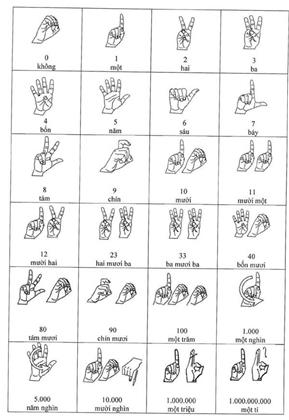
\includegraphics{Images/Theoretical basis/bangso.jpg}
    \caption{Bảng chữ số của ngôn ngữ kí hiệu}
    \label{fig:enter-label}
\end{figure}

\begin{figure}[H]
    \centering
    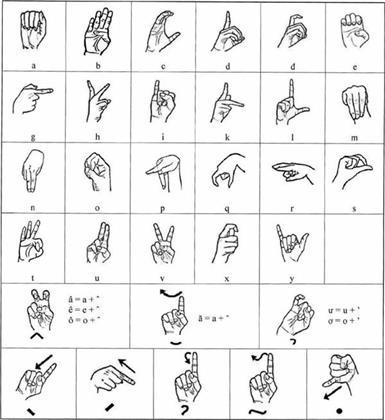
\includegraphics{Images/Theoretical basis/bangchu.jpg}
    \caption{Bảng chữ cái của ngôn ngữ ký hiệu}
    \label{fig:enter-label}
\end{figure}


